\documentclass[a4paper]{llncs}

\title{A static checker for JML's \emph{assignable} clause}

\author{
  N\'estor Cata\~no
\and
  Marieke Huisman
}


\institute{
\email{\{Nestor.Catano, Marieke.Huisman\}@sophia.inria.fr} \\ 
  \inria\ Sophia-Antipolis, France  
}

\newcommand{\defn}[1]{\:\hat{#1}\:}

\newcommand{\lemme}{\textsc{Lemme}}
\newcommand{\inria}{\textsc{Inria}}
\newcommand{\jml}{\textsc{Jml}}
\newcommand{\escj}{\textsc{Esc/Java}}
\newcommand{\eiffel}{\textsc{Eiffel}}
\newcommand{\jass}{\textsc{Jass}}
\newcommand{\jcontract}{\textsc{JContract}}
\newcommand{\loopp}{\textsc{Loop}}
\newcommand{\java}{\textsc{Java}}
\newcommand{\cPP}{\textsc{C/C}\nolinebreak\hspace{-.05em}\raisebox{.4ex}{\tiny\bf
+}\nolinebreak\hspace{-.10em}\raisebox{.4ex}{\tiny\bf +}}
\newcommand{\gplus}{\textsc{GemPlus}}
\newcommand{\ctl}{\textsc{Ctl}}
\newcommand{\pltl}{\textsc{Pltl}}
\newcommand{\csrc}{\textsc{Compaq Src}}
\newcommand{\insPP}{\textsc{Insure\nolinebreak\hspace{-.05em}\raisebox{.4ex}{\tiny\bf
+}\nolinebreak\hspace{-.10em}\raisebox{.4ex}{\tiny\bf +}}}

\newcommand{\modtool}{\texttt{ChAstE}}

\newcommand{\sem}[1]{\ensuremath{\mbox{[\![} {#1} \mbox{]\!]}\/}}

\newtheorem {df}{Definition}

\newcommand{\FullExp}{\(<\)\textsf{Full-exp}\(>\)}
\newcommand{\SufExp}{\(<\)\textsf{Suf-exp}\(>\)}
\newcommand{\Exp}{\(<\)\textsf{Exp}\(>\)}
\newcommand{\Identifier}{\(<\)\textsf{Identifier}\(>\)}
\newcommand{\MethodCall}{\(<\)\textsf{Identifier}\(>\)(\Exp\ldots\Exp)}
\newcommand{\Static}{\(<\)\textsf{StaticClass}\(>\)}
\newcommand{\Type}{\(<\)\textsf{Type}\(>\)}
\newcommand{\option}{\(\:||\)}

\newcommand{\MOD}[2]{\ensuremath{\mathit{#1}\:\mathsf{mod}\:\ensuremath{\mathit{#2}}}}
\newcommand{\MODFE}[2]{\ensuremath{\mathit{#1}\:\mathsf{modFE}\:\mathit{#2}}}
\newcommand{\MODSuf}[2]{\ensuremath{\mathit{#1}\:\mathsf{modSUF}\:\mathit{#2}}}
\newcommand{\MODS}[2]{\ensuremath{\mathit{#1}\:\mathsf{mod}\hspace*{-1.8em}\overrightarrow{\phantom{\mathsf{mop}}}\:\mathit{#2}}}

\newcommand{\method}[2]{\ensuremath{\mathit{#1}\texttt{(}
                                    \overrightarrow{\mathit{#2}}
                                    \texttt{)}}}
\newcommand{\methodx}[2]{\ensuremath{\mathit{#1}\texttt{(}{#2}
                                    \texttt{)}}}
\newcommand{\methodbody}[2]{\ensuremath{\method{#1}{#2}\mathsf{.body}}}
\newcommand{\methodloc}[2]{\ensuremath{\method{#1}{#2}\mathsf{.locvars}}}
\newcommand{\methodassign}[2]{\ensuremath{\method{#1}{#2}\mathsf{.assignable}}}

\newcommand{\actuals}{\textit{actual}\hspace*{-2.6em}\overrightarrow{\phantom{\textit{param}}}}



\newcommand{\extmember}[2]{\ensuremath{#1\: \underline\in\: #2}}
\newcommand{\member}[2]{\ensuremath{#1\: \in\: #2}}
\newcommand{\extsubset}[2]{\ensuremath{#1 \sqsubseteq #2}}

\newcommand{\fieldsof}{\texttt{\(\backslash\)fields\_of}}
\newcommand{\fieldsofarg}[1]{\texttt{\(\backslash\)fields\_of(#1)}}
\newcommand{\reach}{\texttt{\(\backslash\)reach}}
\newcommand{\reacharg}[1]{\texttt{\(\backslash\)reach(#1)}}
\newcommand{\nothing}{\texttt{\(\backslash\)nothing}}
\newcommand{\everything}{\texttt{\(\backslash\)everything}}

\usepackage{lscape} % it's needed to turn a page
\usepackage{amsmath} % it is needed by the \sem command
\usepackage{alltt}
\usepackage{epsfig}

\newcommand{\marginnote}[1]{\marginpar{\framebox{\begin{minipage}{\marginparwidth}{#1}\end{minipage}}}}

\message{<Paul Taylor's Proof Trees, 2 August 1996>}
%% Build proof tree for Natural Deduction, Sequent Calculus, etc.
%% WITH SHORTENING OF PROOF RULES!
%% Paul Taylor, begun 10 Oct 1989
%% *** THIS IS ONLY A PRELIMINARY VERSION AND THINGS MAY CHANGE! ***
%%
%% 2 Aug 1996: fixed \mscount and \proofdotnumber
%%
%%      \prooftree
%%              hyp1            produces:
%%              hyp2
%%              hyp3            hyp1    hyp2    hyp3
%%      \justifies              -------------------- rulename
%%              concl                   concl
%%      \thickness=0.08em
%%      \shiftright 2em
%%      \using
%%              rulename
%%      \endprooftree
%%
%% where the hypotheses may be similar structures or just formulae.
%%
%% To get a vertical string of dots instead of the proof rule, do
%%
%%      \prooftree                      which produces:
%%              [hyp]
%%      \using                                  [hyp]
%%              name                              .
%%      \proofdotseparation=1.2ex                 .name
%%      \proofdotnumber=4                         .
%%      \leadsto                                  .
%%              concl                           concl
%%      \endprooftree
%%
%% Within a prooftree, \[ and \] may be used instead of \prooftree and
%% \endprooftree; this is not permitted at the outer level because it
%% conflicts with LaTeX. Also,
%%      \Justifies
%% produces a double line. In LaTeX you can use \begin{prooftree} and
%% \end{prootree} at the outer level (however this will not work for the inner
%% levels, but in any case why would you want to be so verbose?).
%%
%% All of of the keywords except \prooftree and \endprooftree are optional
%% and may appear in any order. They may also be combined in \newcommand's
%% eg "\def\Cut{\using\sf cut\thickness.08em\justifies}" with the abbreviation
%% "\prooftree hyp1 hyp2 \Cut \concl \endprooftree". This is recommended and
%% some standard abbreviations will be found at the end of this file.
%%
%% \thickness specifies the breadth of the rule in any units, although
%% font-relative units such as "ex" or "em" are preferable.
%% It may optionally be followed by "=".
%% \proofrulebreadth=.08em or \setlength\proofrulebreadth{.08em} may also be
%% used either in place of \thickness or globally; the default is 0.04em.
%% \proofdotseparation and \proofdotnumber control the size of the
%% string of dots
%%
%% If proof trees and formulae are mixed, some explicit spacing is needed,
%% but don't put anything to the left of the left-most (or the right of
%% the right-most) hypothesis, or put it in braces, because this will cause
%% the indentation to be lost.
%%
%% By default the conclusion is centered wrt the left-most and right-most
%% immediate hypotheses (not their proofs); \shiftright or \shiftleft moves
%% it relative to this position. (Not sure about this specification or how
%% it should affect spreading of proof tree.)
%
% global assignments to dimensions seem to have the effect of stretching
% diagrams horizontally.
%
%%==========================================================================

\def\introrule{{\cal I}}\def\elimrule{{\cal E}}%%
\def\andintro{\using{\land}\introrule\justifies}%%
\def\impelim{\using{\Rightarrow}\elimrule\justifies}%%
\def\allintro{\using{\forall}\introrule\justifies}%%
\def\allelim{\using{\forall}\elimrule\justifies}%%
\def\falseelim{\using{\bot}\elimrule\justifies}%%
\def\existsintro{\using{\exists}\introrule\justifies}%%

%% #1 is meant to be 1 or 2 for the first or second formula
\def\andelim#1{\using{\land}#1\elimrule\justifies}%%
\def\orintro#1{\using{\lor}#1\introrule\justifies}%%

%% #1 is meant to be a label corresponding to the discharged hypothesis/es
\def\impintro#1{\using{\Rightarrow}\introrule_{#1}\justifies}%%
\def\orelim#1{\using{\lor}\elimrule_{#1}\justifies}%%
\def\existselim#1{\using{\exists}\elimrule_{#1}\justifies}

%%==========================================================================

\newdimen\proofrulebreadth \proofrulebreadth=.05em
\newdimen\proofdotseparation \proofdotseparation=1.25ex
\newdimen\proofrulebaseline \proofrulebaseline=2ex
\newcount\proofdotnumber \proofdotnumber=3
\let\then\relax
\def\hfi{\hskip0pt plus.0001fil}
\mathchardef\squigto="3A3B
%
% flag where we are
\newif\ifinsideprooftree\insideprooftreefalse
\newif\ifonleftofproofrule\onleftofproofrulefalse
\newif\ifproofdots\proofdotsfalse
\newif\ifdoubleproof\doubleprooffalse
\let\wereinproofbit\relax
%
% dimensions and boxes of bits
\newdimen\shortenproofleft
\newdimen\shortenproofright
\newdimen\proofbelowshift
\newbox\proofabove
\newbox\proofbelow
\newbox\proofrulename
%
% miscellaneous commands for setting values
\def\shiftproofbelow{\let\next\relax\afterassignment\setshiftproofbelow\dimen0 }
\def\shiftproofbelowneg{\def\next{\multiply\dimen0 by-1 }%
\afterassignment\setshiftproofbelow\dimen0 }
\def\setshiftproofbelow{\next\proofbelowshift=\dimen0 }
\def\setproofrulebreadth{\proofrulebreadth}

%=============================================================================
\def\prooftree{% NESTED ZERO (\ifonleftofproofrule)
%
% first find out whether we're at the left-hand end of a proof rule
\ifnum  \lastpenalty=1
\then   \unpenalty
\else   \onleftofproofrulefalse
\fi
%
% some space on left (except if we're on left, and no infinity for outermost)
\ifonleftofproofrule
\else   \ifinsideprooftree
        \then   \hskip.5em plus1fil
        \fi
\fi
%
% begin our proof tree environment
\bgroup% NESTED ONE (\proofbelow, \proofrulename, \proofabove,
%               \shortenproofleft, \shortenproofright, \proofrulebreadth)
\setbox\proofbelow=\hbox{}\setbox\proofrulename=\hbox{}%
\let\justifies\proofover\let\leadsto\proofoverdots\let\Justifies\proofoverdbl
\let\using\proofusing\let\[\prooftree
\ifinsideprooftree\let\]\endprooftree\fi
\proofdotsfalse\doubleprooffalse
\let\thickness\setproofrulebreadth
\let\shiftright\shiftproofbelow \let\shift\shiftproofbelow
\let\shiftleft\shiftproofbelowneg
\let\ifwasinsideprooftree\ifinsideprooftree
\insideprooftreetrue
%
% now begin to set the top of the rule (definitions local to it)
\setbox\proofabove=\hbox\bgroup$\displaystyle % NESTED TWO
\let\wereinproofbit\prooftree
%
% these local variables will be copied out:
\shortenproofleft=0pt \shortenproofright=0pt \proofbelowshift=0pt
%
% flags to enable inner proof tree to detect if on left:
\onleftofproofruletrue\penalty1
}

%=============================================================================
% end whatever box and copy crucial values out of it
\def\eproofbit{% NESTED TWO
%
% various hacks applicable to hypothesis list 
\ifx    \wereinproofbit\prooftree
\then   \ifcase \lastpenalty
        \then   \shortenproofright=0pt  % 0: some other object, no indentation
        \or     \unpenalty\hfil         % 1: empty hypotheses, just glue
        \or     \unpenalty\unskip       % 2: just had a tree, remove glue
        \else   \shortenproofright=0pt  % eh?
        \fi
\fi
%
% pass out crucial values from scope
\global\dimen0=\shortenproofleft
\global\dimen1=\shortenproofright
\global\dimen2=\proofrulebreadth
\global\dimen3=\proofbelowshift
\global\dimen4=\proofdotseparation
\global\count255=\proofdotnumber
%
% end the box
$\egroup  % NESTED ONE
%
% restore the values
\shortenproofleft=\dimen0
\shortenproofright=\dimen1
\proofrulebreadth=\dimen2
\proofbelowshift=\dimen3
\proofdotseparation=\dimen4
\proofdotnumber=\count255
}

%=============================================================================
\def\proofover{% NESTED TWO
\eproofbit % NESTED ONE
\setbox\proofbelow=\hbox\bgroup % NESTED TWO
\let\wereinproofbit\proofover
$\displaystyle
}%
%
%=============================================================================
\def\proofoverdbl{% NESTED TWO
\eproofbit % NESTED ONE
\doubleprooftrue
\setbox\proofbelow=\hbox\bgroup % NESTED TWO
\let\wereinproofbit\proofoverdbl
$\displaystyle
}%
%
%=============================================================================
\def\proofoverdots{% NESTED TWO
\eproofbit % NESTED ONE
\proofdotstrue
\setbox\proofbelow=\hbox\bgroup % NESTED TWO
\let\wereinproofbit\proofoverdots
$\displaystyle
}%
%
%=============================================================================
\def\proofusing{% NESTED TWO
\eproofbit % NESTED ONE
\setbox\proofrulename=\hbox\bgroup % NESTED TWO
\let\wereinproofbit\proofusing
\kern0.3em$
}

%=============================================================================
\def\endprooftree{% NESTED TWO
\eproofbit % NESTED ONE
% \dimen0 =     length of proof rule
% \dimen1 =     indentation of conclusion wrt rule
% \dimen2 =     new \shortenproofleft, ie indentation of conclusion
% \dimen3 =     new \shortenproofright, ie
%                space on right of conclusion to end of tree
% \dimen4 =     space on right of conclusion below rule
  \dimen5 =0pt% spread of hypotheses
% \dimen6, \dimen7 = height & depth of rule
%
% length of rule needed by proof above
\dimen0=\wd\proofabove \advance\dimen0-\shortenproofleft
\advance\dimen0-\shortenproofright
%
% amount of spare space below
\dimen1=.5\dimen0 \advance\dimen1-.5\wd\proofbelow
\dimen4=\dimen1
\advance\dimen1\proofbelowshift \advance\dimen4-\proofbelowshift
%
% conclusion sticks out to left of immediate hypotheses
\ifdim  \dimen1<0pt
\then   \advance\shortenproofleft\dimen1
        \advance\dimen0-\dimen1
        \dimen1=0pt
%       now it sticks out to left of tree!
        \ifdim  \shortenproofleft<0pt
        \then   \setbox\proofabove=\hbox{%
                        \kern-\shortenproofleft\unhbox\proofabove}%
                \shortenproofleft=0pt
        \fi
\fi
%
% and to the right
\ifdim  \dimen4<0pt
\then   \advance\shortenproofright\dimen4
        \advance\dimen0-\dimen4
        \dimen4=0pt
\fi
%
% make sure enough space for label
\ifdim  \shortenproofright<\wd\proofrulename
\then   \shortenproofright=\wd\proofrulename
\fi
%
% calculate new indentations
\dimen2=\shortenproofleft \advance\dimen2 by\dimen1
\dimen3=\shortenproofright\advance\dimen3 by\dimen4
%
% make the rule or dots, with name attached
\ifproofdots
\then
        \dimen6=\shortenproofleft \advance\dimen6 .5\dimen0
        \setbox1=\vbox to\proofdotseparation{\vss\hbox{$\cdot$}\vss}%
        \setbox0=\hbox{%
                \advance\dimen6-.5\wd1
                \kern\dimen6
                $\vcenter to\proofdotnumber\proofdotseparation
                        {\leaders\box1\vfill}$%
                \unhbox\proofrulename}%
\else   \dimen6=\fontdimen22\the\textfont2 % height of maths axis
        \dimen7=\dimen6
        \advance\dimen6by.5\proofrulebreadth
        \advance\dimen7by-.5\proofrulebreadth
        \setbox0=\hbox{%
                \kern\shortenproofleft
                \ifdoubleproof
                \then   \hbox to\dimen0{%
                        $\mathsurround0pt\mathord=\mkern-6mu%
                        \cleaders\hbox{$\mkern-2mu=\mkern-2mu$}\hfill
                        \mkern-6mu\mathord=$}%
                \else   \vrule height\dimen6 depth-\dimen7 width\dimen0
                \fi
                \unhbox\proofrulename}%
        \ht0=\dimen6 \dp0=-\dimen7
\fi
%
% set up to centre outermost tree only
\let\doll\relax
\ifwasinsideprooftree
\then   \let\VBOX\vbox
\else   \ifmmode\else$\let\doll=$\fi
        \let\VBOX\vcenter
\fi
% this \vbox or \vcenter is the actual output:
\VBOX   {\baselineskip\proofrulebaseline \lineskip.2ex
        \expandafter\lineskiplimit\ifproofdots0ex\else-0.6ex\fi
        \hbox   spread\dimen5   {\hfi\unhbox\proofabove\hfi}%
        \hbox{\box0}%
        \hbox   {\kern\dimen2 \box\proofbelow}}\doll%
%
% pass new indentations out of scope
\global\dimen2=\dimen2
\global\dimen3=\dimen3
\egroup % NESTED ZERO
\ifonleftofproofrule
\then   \shortenproofleft=\dimen2
\fi
\shortenproofright=\dimen3
%
% some space on right and flag we've just made a tree
\onleftofproofrulefalse
\ifinsideprooftree
\then   \hskip.5em plus 1fil \penalty2
\fi
}

%==========================================================================
% IDEAS
% 1.    Specification of \shiftright and how to spread trees.
% 2.    Spacing command \m which causes 1em+1fil spacing, over-riding
%       exisiting space on sides of trees and not affecting the
%       detection of being on the left or right.
% 3.    Hack using \@currenvir to detect LaTeX environment; have to
%       use \aftergroup to pass \shortenproofleft/right out.
% 4.    (Pie in the sky) detect how much trees can be "tucked in"
% 5.    Discharged hypotheses (diagonal lines).
 %showing demonstration

\begin{document}
\fussy
\maketitle
\pagestyle{plain}

\begin{abstract}
This paper proposes a syntactic method to check so-called
\emph{assignable} clauses in \java\ programs, annotated with \jml\
assertions. Assignable clauses describe which variables may be
modified by a method. Their correctness is crucial for reasoning about 
class specifications. 

The method that we propose in this paper is incomplete, as it only
does a syntactic check and it does not take aliasing or expression
evaluation into account, but it provides an efficient check that will
find in practice the most common errors in assignable clauses. This is
demonstrated by applying the method to the specification of an
industrial case study.
\end{abstract}






\section{Introduction}
\label{sec-intro}

\paragraph{\bf Formal methods}

%This paper discusses a technique to make the use of formal methods
%easier and more efficient. 
Recently, several light weight approaches to formal methods have
demonstrated that the use of formal methods in practice is actually
feasible~\cite{LeinoNS00,CatanoH02a}.  Up to now, formal methods
merely were considered as a theoretical issue, which could not be
applied to ``real'' problems: the complicated logical notations and
the minimal tool support could not compete with the software
development methods and tools used in industry.

%There are several 
%However, recently this has started to
%change, for several reasons. 
But recently, specification languages have been proposed that closer
resemble programming languages, and powerful tools have been developed
which are tailored to these specification languages. At the same time,
industry has started to feel the need for certified software, in
particular after the discovery of bugs such as in the \textsc{Intel}
\textsc{Pentium II} chips, which costed the company several billion
dollars.


%Several decades ago, the \emph{formal methods} were considered as a merely
%theoretical issue in computer science, not suitable for real
%problems: \emph{complicated} notations taken from the logic and
%the lack of tools supporting formal methods could not compete with the
%tools and methods used in industry for software development. Recently, 
%this has been changing. There are several reasons for this
%change. Firstly, the specification languages are now closer to
%programming languages than ever before and the techniques used are
%more suitable to the actual programming paradigms (object oriented
%and distributed programming). Secondly, industry has started to feel
%the need for certified software. An
%example~\cite{Borger99programmer}: during $1995$,
%\textsc{Intel} found a problem with its microprocessors
%\textsc{Pentium}. This company was forced to replace around two
%million processors. Thus, it realized that the costs of formal
%verification would have been much lower than the costs required to
%fix this bug.

Traditional techniques for program verification are
\textit{model checking} and \textit{theorem proving}. 
Drawbacks of both are that they require a good inside in the
particular verification techniques and tools (\emph{e.g.}~to construct
the model that is input for the model checker or to formalize the
programming language in the logic of the theorem prover), and that
they are often time and memory consuming. By providing a front-end
tool which can translate the program (and possibly also its
specification) automatically into input for the verification tool, the
first drawback partially can be overcome, but when the program does
not satisfy its specification, one still has to understand the problem
in the language of the verification tool.


%Currently, with the interest of the industry and the academic world,
%the developments in formal methods have become
%increased. These developments are specially concerned with techniques
%such as
%\textit{model-checking} and \textit{theorem proving}.
%Model-checking is technique based on constructing a finite model of a
%problem and exhaustively checking the satisfaction of certain
%properties. Model-checking is
%a strong technique, as it is \emph{decidable}, but it presents some
%limitations: $(i)$\ it can validate a
%model of a certain system but not the system itself, and
%$(ii)$\ verification even for simple systems might need huge amounts
%of space and time. 

%Theoretically, interactive theorem proving techniques are able to
%solve any problem proposed in practice, but it presents some
%disadvantages: $(i)$\ it is \emph{undecidable}, $(ii)$\ the tools are
%only capable of assisting an engineer in the process of constructing a
%proof, and $(iii)$\ it requires expressing and understanding the
%semantics underlying the
%programming language in the logic of the theorem prover, in order to
%do program verification. 
%Testing checks whether a program produces
%correct output on certain input. This technique is important for
%checking some properties before applying a formal technique. A
%disadvantage of this approach is that one spends too much of time in the
%process of constructing all possible testing cases. Moreover,
%sometimes it is not possible to check all possible
%inputs. 

Recent tools try to overcome these drawbacks, by using (time and
memory) efficient checking techniques that work directly on the level
of the program and its specification. Two of such techniques are
\textit{run-time checking} and \textit{static checking}. 
These are what could be called light weight formal techniques, which
do not result in a full correctness proof, but can be used to increase
the trust in the correctness of the implementation \emph{w.r.t.}~the
specification, as they are able to find the most common errors.

Run-time checking is a technique where several safety conditions are
checked while running the program, \emph{e.g.}~when making a method
call it is checked that the precondition of the method is not violated
for this particular call, otherwise some error message will be
produced. Typically, run-time checking is implemented by transforming
the program into one that explicitly executes all these
tests. Run-time checking can be seen as extended testing: not only the
input-output behaviour is tested, but also the internal state of the
program at dedicated points. \eiffel~\cite{Meyer97} was the first
programming language which provided this feature (as a special
compiler option). More recent run-time checkers are
\jml~\cite{LeavensBR00} and \jass~\cite{bartetzko01assertions}, 
which check assertions for \java\ programs, and
\insPP~\cite{InsurePP}, which can check memory operations for \cPP
programs. 

%In this paper we will use the specification language of
%\jml.


%a program is transformed into a 
%program which tests several safety conditions at run-time,
%\emph{e.g.}~a program can be transformed so that every time a method 
%is called, it is tested whether the precondition of this method is
%satisfied at the calling point. Typically, if such a condition is
%violated the transformed program will throw an exception, indicating
%which condition was violated at which program point.
%The specification
%language \jml\ that is in this paper ships with a run-time assertion
%checker, which can perform such program transformations.  An important advantage of run-time checking is that
%one does not have to change to another formalism, all the work is done
%at the level of the programming language.

%Other examples of run-time checkers are  A special feature of \jass\ are the
%so-called trace assertions, which allow to check that methods are
%invoked in a prescribed order.

%. This checker keeps track of a \cPP\ program and
%complains whether a block of memory is liberated too many times, a memory
%block is used without being initialized or there exist memory leaks.

%Recently, several approaches have been
%proposed to overcome these kind of problems and although they can not
%actually replace formal verification techniques, they constitute
%important alternatives for checking the behavior of software
%systems. \emph{Run-time
%checking} is a kind of extended checking where, in addition to checking
%the input-output behavior, it is checked whether certain specific
%conditions are
%satisfied at particular points in the program. For checking these
%conditions, the original program is expressed into another
%one
%which can be then executed. If the execution throws an exception,
%this indicates that the original program does not fulfill the
%expected conditions.


Complementary to run-time checking is static checking, where one tries
to find problems in a program by using standard program verification
techniques automatically. Static checking can be considered as an
extended form of type checking, because it finds potential run-time
problems already at compile-time. Typically, static checking gives
quick feedback on a program and can find many common errors, so that
more expensive formal verification techniques can concentrate on the
essential parts of the program. An example of a static checker is
\escj~\cite{LeinoNS00}, which generates proof obligations from an
annotated program and sends these proof obligations to an automatic,
dedicated theorem prover.  


% check the behavior of programs
%from its source code. This technique can be complemented with
%an automatic theorem prover which automatically can detect
%some specific problems. It is expected not to expend too much time in
%this process.

%When using static and run-time checking techniques on software systems,
%it is possible to state
%some specifications which we are interested to check. These
%specifications can be provided to the checking tools as part of the
%source code and written by using a suitable
%specific-specification language. 

\paragraph{\bf{Formal methods for \java}}
Recently, much work on (light-weight) formal methods has focused on
\java\ and \textsc{JavaCard}. Several specification languages have
been developed which are especially tailored to \java, such as
\jass~\cite{bartetzko01assertions} and \jml~\cite{LeavensBR00}.
\jml\ (\java\ \textsc{Modeling} \textsc{Language}) is developed 
by Leavens \emph{et al.}~at Iowa State University. As mentioned above,
together with the specification language a run-time checker is
developed. \jml\ follows the \emph{Design by Contract} approach as
advocated in
\eiffel~\cite{Meyer97}. It allows for example to state pre- and
postconditions of methods and class invariants. \jml\ predicates are
boolean \java\ expressions, extended with some specification-specific
constructs. \jml\ is designed to be easily understandable for a \java\
programmer.

The \jml\ specification language is used as input for several
tools\footnote{With some variations.}. Apart from the \jml\ tool
mentioned above, it is also used as input for the \textsc{Loop}
compiler~\cite{LoopURL,BergJ01}, which translates
\jml-annotated \java\ programs into a series of input theories for the 
theorem prover \textsc{pvs}~\cite{OwreRRSS96}, and for
\escj~\cite{LeinoNS00,EscJmlDiff}. 

\escj\ tries to check an annotated program by
using an automatic, dedicated theorem prover. It is especially tuned
to find errors such as indexing an array out of bounds, null pointer
dereferencing, deadlocks and race conditions, but it also can check
arbitrary functional specifications. If it cannot establish a certain
specification, it issues a warning. As \escj\ neither is sound nor
complete, a warning does not necessarily mean that the program is
incorrect, and no warnings do not necessarily mean that the program is
correct.

%proposed
%for \java\ and \cPP. \jml\ \ (\java\ Model
%Language)~\cite{LeavensBR00} is a tool developed at the Iowa State
%University
%doing run-time checking. Its specification language follows the
%\eiff's approach of \emph{Design by
%Contract}~\cite{Meyer97}, hence
%it is possible to state the functional behavior of methods as
%pre- and postconditions as well as class
%invariants. For
%constructing predicates, in addition to the \java\ boolean operators, 
%\jml\ relies on several logical operators such as the equivalence,
%\texttt{<==>}, and the implication \texttt{==>}, and several
%quantifiers as the existential,
%\texttt{$\backslash$exists}, and the universal, \texttt{$\backslash$forall}.
%Additionally, in \jml\  it is possible to use method
%invocations inside the predicates provide that
%those do not have \emph{side effects}.


%\jass\\  (\java\ With Assertions)~\cite{bartetzko01assertions} is a Design
%by Contract extension for \java\ which allows to annotate
%\java\ programs. The \jass\ tool~\cite{JassUrl} is developed at the
%University of Oldenburg by the group Semantics. \jass\ supports the
%concept of \emph{trace assertions} which are used to monitor the
%dynamic behavior of objects in run-time. This language provides a
%construct called \texttt{changeonly} to specify the list of
%attributes than \emph{may} be modified for a method invocation. This
%list of attributes just consist of identifiers separated by ``.''.

%\escj~\cite{ESCJavaUrl} is a specification language developed at
%\csrc, conceived as a subset of the \jml\ specification
%language~\cite{EscJmlDiff}. The \escj\ tool advocates for doing static
%checking of annotated \java\ programs. Additionally it relies on an
%automatic theorem prover for checking some specific problems. These
%problems cover \texttt{ArrayIndexOutOfBoundExceptions},
%\texttt{NullPointerExceptions} and \emph{Deadlock} and \emph{Race}
%problems in multi-thread \java\ programs.


\paragraph{\bf{Static checking of assignable clauses}}
Within this paper, we develop a static checker which extends \escj, by
checking so-called assignable clauses, \emph{i.e.}~that part of the
specification that states which variables may be changed by a method,
often called frame conditions. The current implementation of \escj\
does not check this~\cite{Leino01,LeinoNS00}.

The checking of methods in \escj\ is done in a modular way, on a
method per method basis.When one encounters a method call in the body
that one is checking, it is not known which method implementation
actually will be called~--~due to dynamic binding. Therefore,
following the behavioral subtype approach~\cite{LiskovW94}, the
method specification in the static class type of the receiver of the
method call will be used\footnote{Additionally, one has to show that
for each overriding method in a subclass, it satisfies the
specification of the superclass.}.

When reasoning in such a way, pre- and postconditions of methods alone 
are not sufficient, one also needs to know which variables may have
been changed by a method. Consider for example the following annotated 
program fragment.

%Recently, several approaches have been
%proposed to overcome these kind of problems and although they can not
%actually replace formal verification techniques, they constitute
%important alternatives for checking the behavior of software
%systems. \emph{Run-time
%checking} is a kind of extended checking where, in addition to checking
%the input-output behavior, it is checked whether certain specific
%conditions are
%satisfied at particular points in the program. For checking these
%conditions, the original program is expressed into another
%one
%which can be then executed. If the execution throws an exception,
%this indicates that the original program does not fulfill the
%expected conditions.

%\emph{Static checking} techniques check the behavior of programs
%from their source code. This technique can be complemented with
%an automatic theorem prover which automatically can detect
%some specific problems. It is expected not to expend too much time in
%this process.

%When using static and run-time checking techniques on software systems,
%it is possible to state
%some specifications which we are interested to check. These
%specifications can be provided to the checking tools as part of the
%source code and written by using a suitable
%specific-specification language. 

%Currently, several specification languages have been proposed
%for \java~and \cPP. \jml~\ (\java~Model
%Language)~\cite{LeavensBR00} is a tool developed at the Iowa State
%University
%doing run-time checking. Its specification language follows the
%\eiff's approach of \emph{Design by
%Contract}~\cite{Meyer97}, hence
%it is possible to state the functional behavior of methods as
%pre- and postconditions as well as class
%invariants. For
%constructing predicates, in addition to the \java~boolean operators, 
%\jml~relies on several logical operators such as the equivalence,
%\texttt{<==>}, and the implication \texttt{==>}, and several
%quantifiers as the existential,
%\texttt{$\backslash$exists}, and the universal, \texttt{$\backslash$forall}.
%Additionally, in \jml~ it is possible to use method
%invocations inside the predicates provide that
%those do not have \emph{side effects}.

%\insPP~is a automatic run-time error detector for
%\cPP~\cite{InsurePP}. This checker keeps track of a \cPP~program and
%complains whether a block of memory is liberated too many times, a memory
%block is used without being initialized or there exist memory leaks.

%\jass\~ (\java~With Assertions)~\cite{bartetzko01assertions} is a Design
%by Contract extension for \java~which allows to annotate
%\java~programs. The \jass~tool~\cite{JassUrl} is developed at the
%University of Oldenburg by the group Semantics. \jass~supports the
%concept of \emph{trace assertions} which are used to monitor the
%dynamic behavior of objects in run-time. This language provides a
%construct called \texttt{changeonly} to specify the list of
%attributes than \emph{may} be modified for a method invocation. This
%list of attributes just consist of identifiers separated by ``.''.

%\escj~\cite{ESCJavaUrl} is a specification language developed at
%\csrc, conceived as a subset of the \jml~specification
%language~\cite{EscJmlDiff}. The \escj~tool advocates for doing static
%checking of annotated \java~programs. Additionally it relies on an
%automatic theorem prover for checking some specific problems. These
%problems cover \texttt{ArrayIndexOutOfBoundExceptions},
%\texttt{NullPointerExceptions} and \emph{Deadlock} and \emph{Race}
%problems in multi-thread \java~programs. \escj~neither is sound nor
%complete, hence whether it issues a warning it does not necessary
%means that some problem occurs. \escj~ships with a specific construct,
%\texttt{modifies}, for specifying the \emph{assignable} behavior of a
%method, but unlike the \jass~tool the variable locations one can
%annotate as assignable can become intricate. Thus, it is possible,
%for instance, to state as assignable all elements of some array
%(\texttt{a[$*$]}) or the fields of some object
%expression $e$ (\texttt{fields\_of($e$)}). \escj~tool does not check
%the correct specification of the assignable behavior of a method,
%hence some verifications problems arise.
%%The annotation language for \eiff~is the first
%%example of such a specification language, following the \emph{design
%%by contract} approach~\cite{Meyer97}. 



%\paragraph{\bf The side-effects freeness problem.}
%The functional behavior as can be expressed by pre- and postconditions
%is not enough to reason about arbitrary method invocations. Suppose we 
%have the example presented below. 
\begin{alltt}
public class C\verb!{!
  int[] arr;

  //@ ensures arr.length >= 4;
  public void m()\verb!{!arr = new int[5]; n();\verb!}!

  //@ ensures true;
  public void n()\verb!{!arr = new int[2];\verb!}!
\verb!}!
\end{alltt}
To establish whether \texttt{m} will satisfy its postcondition, the
functional specification of \texttt{n} alone does not give enough
information, one also needs to know whether \texttt{n} might change
the variable \texttt{arr}. Therefore, \jml\ and \escj\ allow the user
to specify a so-called assignable clause~--~using the keyword
\texttt{modifies}\footnote{\jml\ also allows the alternative keywords
\texttt{assignable} and \texttt{modifiable}.}~--~specifying a set of
locations (typically variables) that may be modified by a method. An
assignable clause can contain variable names, but also more
complicated expressions, \emph{e.g.}~to denote all the elements in an
array or all the fields of an object. By default, when a method
specification does not contain an assignable clause, the method is
supposed to modify nothing. %\jml\
%even allows more general expressions to
%occur in the assignable clause.

The current version of \escj\ does not check assignable clauses, it
only uses them when checking method calls.  As specifying assignable
clauses is error-prone and the information in the assignable clause is
crucial in the verification of other methods, we think this is a
significant omission. When specifying a real-life application it is
easy to forget to mention some variables in the assignable
clause~--~see for example our experiences with the specification and
static checking of an industrial case study~\cite{CatanoH02a} in
Sect.~\ref{sub-sec-usi-the-too}. Therefore, in this paper we propose a
method to do static checking of assignable clauses.


%Therefor

%e, we think it is important that assignable clauses are
%checked, b
%An incorrect assignable clause can cause
%other incorrect method specifications to be accepted, which can then cause
%other incorrect method specifications to be accepted, and so
%on... 
% But Therefore, it is important to have a tool
%which checks assignable clauses, even when it is only on a syntactic
%basis, without taking aliasing into account. Such a tool is presented
%in this paper.


The method works on a syntactic basis. For every method, and for every
assignment\footnote{And for all syntactic variations of assignments.}
in this method we check whether it may violate the assignable clause
of the method. Also, for every method call encountered in a method
body, it is checked whether this method call agrees with the
assignable clause of the body that is checked. We have implemented a
tool performing all the checks automatically.

Our method is neither sound nor complete, for example because it does
not handle aliasing and because it does not keep track of variable
updates\footnote{For example, for a program fragment \texttt{\{i++;
a[i] = 3;\}} it will accept an assignable clause \texttt{modifies
a[i];}.}. However, our experiments show that in practice our method is
very useful, because it finds immediately the most common mistake in
an assignable clause: forgetting completely to mention that a variable
may be modified.  We feel that when specifying a method in which
variables are modified in a complicated or tricky way, a specifier
will be careful when writing the assignable clause and will be more
willing to do full verification, while for simple methods he is more
likely to forget to mention some variables and does not want to
use full verification to detect this.

%The functional behavior of \texttt{n} is not enough to \emph{ensure}
%the post-condition of \texttt{m}, \emph{i.e.}, to ensure that the
%length of \texttt{arr} still will be greater or equal than $4$ after
%the invocation of \texttt{n}. Hence, it arises the need of specifying
%the \emph{changeable} behavior of methods,\emph{i.e}, of specifying what
%is set of variables locations a certain method modifies.



%\escj\ ships with a specific construct,
%\texttt{modifies}, 


%for specifying the \emph{assignable} behavior of a
%method, but unlike the \jass\ tool the variable locations one can
%annotate as assignable can become intricate. Thus, it is possible,
%for instance, to state as assignable all elements of some array
%(\texttt{a[$*$]}) or the fields of some object
%expression $e$ (\texttt{fields\_of($e$)}). \escj\ tool does not check
%the correct specification of the assignable behavior of a method,
%hence some verifications problems arise.


%\paragraph{\bf This paper.}We propose a static checker for the correct
%specification of the
%\emph{assignable} (as a subset of \emph{modifiable}) behavior of
%\jml\ annotated programs. For this purpose, we define a set
%of rules for each \java\ construct which state the variable locations
%these instructions \emph{may} modify. This checker carries out an
%syntactical analysis of the source program and checks whether its
%methods declarations fulfill their assignable specifications. By using
%these rules one can detect errors such as
%declaring a method without \emph{side-effects} when it actually modifies 
%some variable location. Our rules are neither sound nor complete
%(following the \escj\ approach), as we can not detect the most subtle
%errors since they require a detailed analysis, but using them the
%most simple errors can be detected quickly. We have developed the tool
%\modtool\ which implements these rules, by using the Abstract syntax
%tree generated by the parser of \jml. The feasibility of our approach is
%shown by presenting some gaps found in the process of checking the
%specification of the
%assignable behavior of a realistic case study~\cite{CatanoH02a}.

\paragraph{\bf{Related work}}
The term \emph{frame condition} finds its origins in the field of
AI~\cite{McCarthyH69}. Borgida \emph{et al.} revealed the relationship
with formal specifications, where one needs to know which part of the
state may be modified. They discuss several approaches, and finally
propose to use so-called change axioms which can describe the possible
changes of the state under a certain condition. They also give a
syntactic method which can be used to generate a first attempt for the
change axioms. A limitation of their approach is that they only look
at single variables, while we can also handle expressions describing a
set of memory locations.

Leino~\cite{Leino98} and M\"uller~\cite{Mueller01} both studied
how to specify and verify assignable clauses in subclasses and/or
using abstract variables. In this paper we only look at assignable
clauses containing concrete variables. When extending our work to
abstract variables, their work would form the basis to deal with
dependencies. 

Within the \jass\ project~\cite{JassUrl} the non-violation of assignable
clauses can be checked at run-time, but this is restricted to simple
variables only, more complex expressions are not allowed in the
assignable clauses.

Finally, within the \loopp\ project a \emph{semantic} definition for
assignable clauses is defined. When verifying a method body, one has
to show that each variable not mentioned in the assignable clause is
unchanged. This is a heavy proof burden, because it involves
quantifications over the whole state. Therefore, it is useful to first
check automatically whether the assignable clause is likely to be
correct, before diving into the full verification.

\paragraph{\bf{Organization}}

The rest of this paper is organized as follows.
Sect.~\ref{sec-esc-prg} briefly presents the most important
assertion constructs of \jml\ and \escj. Sect.~\ref{sec-ass}
discusses the meaning of the assignable clause.
Sect.~\ref{sec-syn-met-che-ass-cla} presents the rules that we use
to check assignable clauses, and Sect.~\ref{sec-che-for-ass-cla}
presents our implementation on top of the \jml\ parser and discusses
practical experiences.  Finally, Sect.~\ref{sec-con-and-fut-wor}
gives conclusions and presents future work.






\section{JML and ESC/Java specifications}
\label{sec-esc-prg}
%\escj\ is a static checker for \java\ programs developed
%at \csrc~\cite{ESCJavaUrl}, allowing a user to find common programming
%errors, such as nullpointer exceptions, array index out of bound
%exceptions, deadlocks and race conditions. It does this by generating
%appropriate proof obligations and sending these off to an automatic,
%dedicated theorem prover. A user can specify additional class and
%method specifications (\emph{e.g.}~class invariants, pre and post
%conditions), which the tool will also try to check.  If the underlying
%theorem prover cannot establish a certain proof obligation, the tool
%issues a warning. Such a warning does not necessarily mean that the
%program is wrong, since the \escj\ approach is neither sound nor
%complete. \escj\ expressions are boolean \java\ expressions, extended
%with several specification-specific constructs. 

%It relies on a dedicated theorem prover to
%find specific problems
%The basic idea is that
%a user specifies the behavior of a class and its methods, by
%using the specification language of \escj. This
%behavior can be expressed as \textit{preconditions},
%\textit{postconditions} and \textit{class invariants}. The \escj\ tool
%checks whether the implementation satisfies the given
%specification and 

The \jml\ specification language is designed to be 
easily usable for \java\ programmers. In particular, \jml\ expressions
are side-effect free boolean \java\ expressions, extended with some
specification-specific constructs. The specification language for
\escj\ uses the same design principles. Initially there were several
differences between the two languages, but to enable the use of
different tools on the same specification, effort has been put in
making the two languages converge~\cite{EscJmlDiff}. In this paper, we 
do not really distinguish between the two languages\footnote{In
particular, we do not consider \jml's model variables.}, although we
take the more general \jml\ format for assignable clauses.

Below, we briefly present the main \jml\ and \escj\ constructs,
followed by a simple method specification example. A complete
description can be found in~\cite{LeavensBR00,LeinoNS00}.
\begin{itemize}
\item[] \textbf{Constructs for specifying methods:} 
\begin{itemize}
\item[-]{\texttt{requires P}: precondition {\tt P};}
%This construct specifies a precondition {\tt P}. 
%When \escj\ checks the body of a
%method, it assumes that \texttt{P} holds initially and when checking
%a method call, it will issue a warning if 
%it can not establish that \texttt{P} holds at the call point. 
 
\item[-]{\texttt{ensures Q}: postcondition {\tt Q};} 
%This construct specifies a postcondition \texttt{Q}. This postcondition
%is checked against the body of method and assumed for any method
%invocation if the method terminates normally (without throwing an
%exception).
 
\item[-]{\texttt{exsures (E) R}: exceptional postcondition \texttt{R},
\emph{i.e.}~if the method terminates abruptly with an exception in
\texttt{E}, then \texttt{R} should be satisfied; }
%This construct specifies an exceptional condition \texttt{R}. This
%condition is
%supposed to hold if the method finishes abruptly and if
%the exception \texttt{e} that is thrown is a subclass of \texttt{E}. 

\item[-]{\texttt{modifies L}: locations \texttt{L} that
a method may modify (see Sect.~\ref{sec-ass}).}
 
\end{itemize}
 
\item[] \textbf{Specification expressions}  
 
\begin{itemize} 
\item[-]{\texttt{==>}, \texttt{<==>}, \texttt{<=!=>}}: logical
implication, equivalence and non-equivalence;
%So, \texttt{P 
%==> Q} is true if and only if \texttt{P} is false or \texttt{Q} is 
%true, where \texttt{P} and \texttt{Q} are specification expressions of  
%\texttt{boolean} type. Furthermore, \texttt{<==>} represents the logical
%equivalence and \texttt{<=!=>} specifies non-equivalence. 
 
\item[-] {($\backslash$\texttt{forall T V; E)}, 
($\backslash$\texttt{exists T V; E})}: universal and existential
quantification;
% are quantifier expressions (of 
%type \texttt{boolean}).  The first expression denotes that \texttt{E}
%is true
%for all substitutions of values of type \texttt{T} for the bound 
%variable \texttt{V}. The second one denotes that \texttt{E} is true 
%for a substitution of a value of type \texttt{T} for the bound 
%variable \texttt{V}. 
 
\item[-]{\texttt{$\backslash$old(E)}}: 
value of expression \texttt{E} in pre-state of method
(in postcondition only);
 
\item[-] {\tt$\backslash$result}: method return value (in postcondition
only).
%returned by 
%a non-void method. It can only be used within an
%\texttt{ensures} clause.
\end{itemize} 
\end{itemize} 

As an example of a method specification, we give the
specification of the method \texttt{addCurrency} from an electronic
purse case study~\cite{CatanoH02a}. This specification has been
checked with \escj.
%A typical annotation example using 
%\escj. This example was taken from the formal specification of an
%\emph{electronic purse} as presented in~\cite{CatanoH02a}\footnote{The whole
%specification can be taken
%from~\cite{CatanoH01URL}.}. 
%%%%%%%
\begin{alltt}
/*@
  modifies nbData, data[nbData];
  ensures (\verb!\!old(nbData) < MAX_DATA) ?
      (nbData == \verb!\!old(nbData) + 1 && data[\verb!\!old(nbData)] == cur) :
      (nbData == \verb!\!old(nbData));
*/
void addCurrency(byte cur)\verb!{!
   if(nbData < MAX_DATA)\verb!{!data[nbData] = cur; nbData++;\verb!}!
\verb!}!
\end{alltt}
%%%%%%%%
The \texttt{addCurrency} method belongs
to a class \texttt{Currencies}, storing all currencies 
supported by the purse application. The method 
\texttt{addCurrency} adds a new currency to the list of valid 
currencies (the array \texttt{data}). The \texttt{modifies} clause
specifies that this method may modify only \texttt{nbData} and 
\texttt{data} in the position \texttt{nbData}. The
postcondition of the method \texttt{addCurrency} (written as 
\texttt{ensures} clauses) expresses that if \texttt{nbData} has not 
yet reached the threshold value \texttt{MAX$\_$DATA}, \texttt{nbData} 
will increase its value by one and the value of the formal parameter 
\texttt{cur} will be assigned to
\texttt{data[\(\backslash\)old(nbData)]}, otherwise \texttt{nbData} is 
unchanged.  Inside the postcondition, the expression
\texttt{$\backslash$old(nbData)} refers to the value of 
\texttt{nbData} before the method invocation. 

\begin{figure}[tb]
\begin{tabular}{rcl}
%$<$\textsf{Assignable-spec}$>$ &::= &$<$\textsf{Assignable-clause}$>$ $<$\textsf{Assignable-exps}$>$ \\
%$<$\textsf{Assignable-exps}$>$ &::= &$<$\textsf{Assignable-exp}$>$\texttt{,}$<$\textsf{Assignable-exps}$>$ $|| $\\
%                           &    &$<$\textsf{Assignable-exp}$>$ \\

$<$\textsf{Assignable-exp}$>$  
  & ::=  & $<$\textsf{Identifier}$>$ \\
  &$\mid$& $<$\textsf{Identifier}$>$\texttt{[}\textsf{Exp}\texttt{]} \\
  &$\mid$& $<$\textsf{Identifier}$>$\texttt{[}\textsf{Exp}\ldots \textsf{Exp}\texttt{]}  \\
  &$\mid$& $<$\textsf{Identifier}$>$\texttt{[}*\texttt{]} \\
  &$\mid$& $\backslash$\texttt{fields\_of(}$<$\textsf{Field-exp}$>$\texttt{)}  \\
  &$\mid$& $\backslash$\texttt{nothing} \\
  &$\mid$& $\backslash$\texttt{everything} \\

$<$\textsf{Field-exp}$>$ 
  & ::=  & $<$\textsf{Point-identif}$>$  \\
  &$\mid$& \texttt{this} \\
  &$\mid$& $\backslash$\texttt{reach(}$<$\textsf{Point-identif}$>$\texttt{)}  \\
  &$\mid$& \texttt{reach(}\texttt{this}\texttt{)}  \\

$<$\textsf{Point-identif}$>$   
  & ::=  & $<$\textsf{Identifier}$>$\texttt{.}$<$\textsf{Point-identif}$> $ \\
  &$\mid$ & $<$\textsf{Identifier}$>$ \\
%$<$\textsf{Assignable-clause}$>$ &::= &\texttt{assignable}   \\
%                             &    &\texttt{modifiable}   \\
%                             &    &\texttt{modifies} \\
\end{tabular}
\caption{Syntax for an assignable expression}\label{FigAssignableExpr}
\end{figure}


\section{JML's assignable clauses}
\label{sec-ass}

An assignable clause specifies which variables may 
be modified by a method; all other variables \emph{should} remain
unchanged. Within an assignable clause, a list of so-called assignable 
expressions is specified which describe which memory locations may be
modified. The exact syntax for an assignable
expression is given in Fig.~\ref{FigAssignableExpr}.

%The syntax of specification of a assignable clause in a
%\java\ annotated program
%is presented by the figure~\ref{fig-syn-mod-spe}. 

An assignable expression can be an identifier or a simple array
indexing expression denoting a single location, but it can also denote
a set of locations. An expression
\texttt{a[i\dots j]} denotes the set of locations
\(\{\texttt{a[}k\texttt{]}\mid \texttt{i} \leq k \leq \texttt{j}\}\), while
\texttt{a[*]} denotes the same set as \texttt{a[0\dots a.length - 1]}.
An assignable expression \fieldsofarg{\(e\)} denotes the set of
\emph{all fields} of the objects represented by the expression \(e\).
The expression \(e\) can be a single object (again possibly
\texttt{this}), or it is the \reach\ of some object \(f\) (possibly
\texttt{this}). The expression \reacharg{\(f\)} denotes the minimal 
set containing \(f\), the fields of \(f\) and all objects reachable
from the fields of \(f\).  Finally, there are special keywords
\nothing\ and \everything, denoting the empty set of locations and the 
full set of locations, respectively.

%collection of
%variable of reference type, and where
%\texttt{$\backslash$fields\_of(x)} denotes all fields of \texttt{
%denotes \texttt{x[*]} if \texttt{x}
%is an array, otherwise the set of fields of \texttt{x}. The construct
%\texttt{$\backslash$reach} only can occur inside a \texttt{fields\_of}
%construct. An specification like \texttt{$\backslash$reach(x)} denotes
%the minimal set containing \texttt{x}, the fields of \texttt{x} and
%all objects
%reachable from the fields of \texttt{x}. A specification like
%\texttt{modifies \!\!$\backslash$nothing} expresses the method as not
%having
%side-effects. Additionally, a specification like \texttt{modifies
%\!\!$\backslash$everything} expresses that the method may modify any
%variable location.
%%%%%%%%%%%%%%%%%%
%%%%%%%%%%%%%%%%%%%%
%We present a set of syntactical rules which check the correct
%specification of assignable clauses in \java\ asserted programs. These
%rules have been defined taking into account both of the \jml\ grammar
%%specification and the definition of assignable clauses presented
%in~\cite{LeavensBR00}.

Given the set of locations characterized by the assignable
expressions, a \jml\ assignable clause is defined as
follows\footnote{This definition differs
from~\cite{LeavensBR00} in that it does not consider dependencies, 
as we do not consider model variables.}.
%We present the definition concerning the conditions about the assignment
%of expressions in \jml. This definition was taken directly
%from~\cite{LeavensBR00}.
\begin{definition}[Assignable clause]
\label{def-mod}
An \emph{assignable clause} only allows a method to modify a location
\emph{loc} if:
\begin{itemize}
\item \emph{loc} is mentioned in the method's assignable
clause;
\item \emph{loc} is not allocated when the method starts execution; or
\item \emph{loc} is local to the method (\emph{i.e.}, a local
variable or a formal parameter).
\end{itemize}
\end{definition}

Notice that this is a syntactic definition, thus an assignment
\texttt{x = x;} only is permitted if the 
variable \texttt{x} is mentioned in the appropriate assignable clause
or if \texttt{x} is a local variable.

When overriding a method in a subclass, \jml\ allows one only to
extend the assignable clause of the overridden method. To reduce the
possibilities of unsoundness in modular verification, the assignable
clause in the subclass preferably only adds variables (or expressions)
that are not visible in the scope of the overridden
method~\cite{LeinoNS00,Leino98}.

%To ensure that a method implementation respects its assignable clause, 
%one should state proof obligations of the form \(s\:\mathsf{mod}\:A\),
%for each instruction \(s\) in the method, where \textsf{mod} is
%defined as follows\footnote{Notice that 

%meaning \(s\) may only modify the variables
%denoted by \(A\).


%We have adapted this definition in the presentation of our \textsf{mod}
%rules. Thereby the definition~\ref{df-mod}.
%%%%%%%%%%%%%%
%\begin{definition}[\textsf{mod}]
%\label{df-mod}
%\[s\:\mathsf{mod}\:A \defn{=} \forall x \in LC.\,x \not\in A \Rightarrow 
%\textit{Pre}_s(x) = \textit{Post}_s(x)\]
%%$s$\ \textsf{mod}~$A$ $\Leftrightarrow$ $\forall x \in LC.\,
%%x\not\in$ \textsc{A}$\ \Rightarrow Pre(x) = Post(x)$ \\
%where $LC$ is a set of variable locations, $s$ is some
%instruction, $\textit{Pre}_s(x)$
%refers to the value of $x$ before executing $s$,
%$\textit{Post}_s(x)$ refers to the value of $x$ after executing
%$s$ and $A$ is the set of variables that may be modified by \(s\).
%\end{definition}



%This section 


%We present a set of syntactical rules which define the conditions that
%must be fulfilled for any instruction occurring in a
%\java\ annotated program. We have profited the syntax of \java\ for
%defining our rules. Thus, for instance, we rely on rules for
%expressions, statements, and so on. The basic idea is that for each
%sort of instruction occurring in a method
%declaration, these rules check that the variable locations they assign
%belongs to the set of variable locations that the
%method \emph{may} modify.


%The rest of this section is organized as it follows. Sect.
%\ref{sub-sec-ass-beh} present the syntax of specification of
%assignable clause and certain other definitions used in the
%specification of our rules. Sections \ref{sub-sec-rul-con-met},
%\ref{sub-sec-rul-con-pri-suf-and-pri-exp}, \ref{sub-sec-rul-con-ass},
%\ref{sub-sec-rul-con-ope}, \ref{sub-sec-rul-con-sta}, and
%\ref{sub-sec-tra-rul} present the rules for the different
%\java\ constructs. Section \ref{sub-sec-the-rel-mem} the definition of
%membership operator used in the specification of our rules.






%\subsection{Assignable Behavior}
%\label{sub-sec-ass-beh}


%%%%%%%%%%%%%%
%These \textsf{mod} rules have beeing reformulated in other more
%specific ones, considering the syntactical structure of
%\java. Consequently, we rely on \textsf{modEXP} for
%expressions, \textsf{modSTM} for statements and so on. 
%on so-called primary
%expressions (


\section{A syntactical method to check assignable clauses}
\label{sec-syn-met-che-ass-cla}

This section presents a syntactic method to derive for each method
whether it does not violate its assignable clause. In particular, for
each assignment and for each method call, appropriate checks are defined.


\subsection{Preliminaries}
For each language construct \(s\) we will define a rule which allows
us to derive the correctness of \MOD{s}{A}, with the intuitive
meaning: statement \(s\) only assigns to variables which are mentioned
in assignable clause \(A\). Together, these rules exactly define
\textsf{mod}.

In some cases we need to lift \textsf{mod} over a set of
instructions. Therefore, we define the following.

\begin{definition}[$\overrightarrow{\textsf{mod}}$]
\label{def-mod-lis}
Given \(S\) a set of statements and \(A\) an assignable clause,
\(\mathsf{mod}\) is \emph{lifted} over the set of instructions as follows.
\[\MODS{S}{A} \defn{=}\forall s.\,s\in S\Rightarrow \MOD{s}{A}\]
%$S\ \overrightarrow{\textsf{mod}}~A$ iff $\forall s.\ s\in
%S\Rightarrow s\ \textsf{mod}~A$
\end{definition}

As mentioned in the previous section, the assignable clause can
contain expressions as
\fieldsofarg{this}, thus checking whether a
variable occurs in the assignable clause cannot be done by simply using set
membership \(\in\). Therefore, we use an extended notion of set
membership, subsuming \(\in\), denoted by \(\underline\in\). Below, in 
Subsection~\ref{sub-sec-the-rel-mem} this notion is defined precisely.

Based on the notion of extended set membership, we can also define the
notion of an \emph{extended membership subset}.
%Each rule
%checks that the set of locations modified by the corresponding
%instruction \emph{belongs} to a set of locations specifined as modified for
%the method. This concept $\underline\in$ of membership must be
%formulated considering
%the syntaxis of the assignable declarations (see
%Fig.~\ref{fig-syn-mod-spe}), but intituivaly subsumes the standard
%concept $\in$. Sect.~\ref{sub-sec-the-rel-mem} shows the definition
%of this concept. 

%Once we count on the definition of membership for assignable
%locations, we should give the definition for the
%inclusion. Figure~\ref{def-subseq} presents the definition of inclusion of
%assignable locations.
%%%%%%%%%%
\begin{definition}[Extended membership subset $\sqsubseteq$]
\label{def-subseq}
Given assignable clauses \(A_1\) and \(A_2\) the \emph{extended
membership subset} predicate is  defined as follows.
\[\extsubset{A_1}{A_2} \defn{=} \forall v.\ \extmember{v}{A_1}
\Rightarrow \extmember{v}{A_2}\]
\end{definition} 


We will also define variant notions \textsf{modFE} and
\textsf{modSUF}, with a similar intuitive meaning, but
defined only on so-called \emph{full expressions} and \emph{suffix
expression}, respectively.

%Notice that \textsf{mod} is
%a syntactic notion, and we cannot give a semantic definition for
%it\footnote{In particular, a semantic definition would never be able
%to find that \texttt{x = x;} could violate an assignable clause.}, but 
%the rules presented below together define 

\begin{figure}[tb]
\begin{tabular}{lr}
\begin{tabular}[t]{rcl}
\FullExp & ::=  & \FullExp[\Exp\(^+\)]  \\
         &$\mid$& \FullExp(\Exp\(^*\))  \\
         &$\mid$& \FullExp.\SufExp  \\
         &$\mid$& \SufExp\\
\\
\end{tabular}
&
\hspace*{2em}
\begin{tabular}[t]{rcl}
\SufExp  & ::=  & \Identifier  \\
         &$\mid$& \texttt{this}  \\
         &$\mid$& \texttt{super}  \\
         &$\mid$& \textsf{Literal}\\
         &$\mid$& \texttt{new} \Type [\Exp]\\
         &$\mid$& \texttt{new} \Type (\Exp\(^*\))\\
%\FullExp & ::= & \FullExp.\SufExp \option \\
%              && \textsf{Literal} \option \\ && \texttt{new}
%              \Type(\Exp) \option \\ && \texttt{new} \Type[\Exp]
%              \option \\ && \FullExp.\MethodCall \option \\ &&
%              \MethodCall \option\\ && \SufExp \\
%\\
%\SufExp & ::= & \Identifier \option \texttt{super} \option
%                \texttt{this} \option \Static \option
%                \Identifier[\Exp]\\
\end{tabular}
\end{tabular}
\caption{Syntax for full expressions and suffix expressions}
\label{FigExpGrammar}
\end{figure}

Full expressions and suffix expressions are defined following the
syntax in Fig.~\ref{FigExpGrammar}. A full expression is an array
indexing expression, a method call, a qualified expression or a suffix
expression. A suffix expression can be an identifier, a reference to
\texttt{super} or \texttt{this}, a literal or an initialization of an 
object or array.  This syntax is a simplified version of the
\jml\ and \java\ grammar~\cite{LeavensBR00,GoslingJSB00}, because we 
assume that the program is accepted by the \java\ compiler and/or the
\jml\ tool.% Thus, we can rely on the fact that the syntax will obey
%this grammar.
We assume that we have predicates \textsf{full?} and
\textsf{suffix?} which can decide whether an expression is a full
expression or a suffix expression, respectively.


%%%%%%%%%%
%Definition~\ref{def-mod-lis} generalize the concept introduce by
%Definition~\ref{df-mod}, by extending it for set of instructions.
%%%%%%%%%
%%%%%%%%%%

%We have also introduced some other \emph{mod}
%constructs by exploiting the \java\ syntax. These \emph{mod}
%constructs cover concepts such as \textit{modSTM}, \textit{modEXP},
%\textit{modPE}, \textit{modPRM} and \textit{modPS}, which redefine the
%original concept \textit{mod} in terms of concepts for
%\emph{statements}, \emph{expressions}, \emph{post-expressions},
%\emph{primary} and \emph{suffixes} expressions respectively. A primary
%\java\ expression can be seen as the first expression in a
%sequence of \java\ expressions joined by the symbol \texttt{``.''}. All 
%of the other expressions make up the suffix of the original
%expression.
%
%expresses that if the set of assignable variable locations of certain
%method is represented by locations $A$, then this method may modify the set
%of expressions \textsc{A}, and in its method body occur expressions or
%declarations such as \textup{f}$_1$\textup{(e}$_1$\textup{,
%f}$_2$\textup{(e}$_2$\textup{,}$\cdots$
%\textup{(f}$_n$\textup{(e}$_n$\textup{))))}, then their correctness
%will be established in terms of the correctness of each subexpression
%\textup{e}$_i$ \emph{w.r.t} \textsc{A}. 




\subsection{The rules defining \textsf{mod}, \textsf{modFE} and \textsf{modSUF}}
For each language construct, appropriate rules are given to define
\textsf{mod}, \textsf{modFE} and \textsf{modSUF} in a compositional
way.  In several cases, the
\java\ and \jml\ syntax prescribes that a certain subexpression of an 
arbitrary expression is a so-called full expression (see
Fig.~\ref{FigExpGrammar}) or that a subexpression of a full expression
is a suffix expression. Therefore, \textsf{mod} will be defined in
terms of \textsf{modFE}, and \textsf{modFE} will be defined in terms
of \textsf{modSUF}.

\subsubsection{Method rules}
\label{sub-sec-rul-con-met}
%We have defined certain syntactical rules for every \java\ construct,
%stating which variables may be modified. Our rules check for
%all \java\ constructs that the expressions modified by instructions
%inside all method bodies are according to
%their assignable specification. We present the derivation rules for
%the most important \java\ constructs. The whole set of rules can be found
%in~\cite{CatanoMasterThesis01}.
The first rules that we define are related with methods. For each
method we check that the assignable clause is respected by the method
body~--~assuming that the assignable clauses for all methods called
from this method body are correct.  Following
Def.~\ref{def-mod}, it is sufficient to check that a method body
only modifies its local variables or formal parameters or 
the variables mentioned in its assignable clause \(A\).


%\textsf{Meth-Dec} is the rule corresponding to a method declaration
%\texttt{m(}$\overrightarrow{\texttt{o}}$\texttt{)} that has
%specified may modify the set of variable locations $A$. This rule
%states that for this method declaration, it is enough to
%check every instruction in its method body
%(\texttt{m(}$\overrightarrow{\texttt{o}}$\texttt{).body}) with respect
%to \textsc{A}, the set of parameters and the local variables to the
%method. As can be seen, this rule essentially formalizes
%Definition~\ref{def-mod}. 
%%%%%
\[
\begin{tabular}{ll}
\textsf{(Meth-Dec)}\,\,\,&
\begin{prooftree} 
\MOD{\methodbody{m}{param}}{(A \cup \{\overrightarrow{\textit{param}}\}
                           \cup \{\methodloc{m}{param}\}) }
\justifies
\MOD{\method{m}{param}}{A}
\end{prooftree}
\end{tabular}
\]
%%%%%

When encountering a method invocation, its assignable clause should be
a subset of the assignable clause \(A\) of the method body that is
currently checked~--~with appropriate substitutions~--~to ensure that
no other variables than the ones mentioned in \(A\) are changed.
According to the \jml\ grammar, method invocations are always full
expressions, thus there is only a rule defining \textsf{modFE}.
Following the syntax in Fig.~\ref{FigExpGrammar}, a method invocation
will be of the form \(\method{fe}{param}\) where \textit{fe} is a full
expression again. Given that the expression is accepted by the \java\
compiler, \textit{fe} will be a qualified expression
\(<\)\textsf{Full-exp}\(>\).\(<\)\textsf{Suf-exp}\(>\), or it will be 
a suffix expression only. The suffix expression must be a method name,
\texttt{this} or \texttt{super}. The appropriate assignable clause can 
be found by looking at the static type of the receiving object of the
method call (possibly \texttt{this}).  This is sufficient, provided
that additional assignable clauses in overriding methods do not name
locations that are visible in the scope of the overridden
method~\cite{LeinoNS00,Leino98}.

Additionally it should be checked that the full expression
\textit{fe} and the actual parameters do not violate the assignable
clause \(A\).


%A method invocation
%$e\texttt{.m(}\overrightarrow{\texttt{q}}\texttt{)}$,
%must fulfill the assignable specification corresponding to its
%method declaration $\texttt{m(}\overrightarrow{\texttt{o}}\texttt{)}$
%previous replacing: $(i)$\ \texttt{this} by $e$ and
%$(ii)$\ $\overrightarrow{\texttt{o}}$ by
%$\overrightarrow{\texttt{q}}$. Additionally, the actual parameters
%$\overrightarrow{\texttt{q}}$ must be checked for
%side-effects. It similar to the expression $e$ (see rule
%\textsf{Meth-Inv}). As can be seen this rules use \textsf{modEXP}
%and \textsf{modPE} rules. \textsf{modEXP} stands for expressions and
%\textsf{modPE} for post-fix expressions. A \java\ post-fix
%expression represents a sort of \emph{primary} expressions linked by
%``.''. A typical primary \java\ expression is a \java\ identifier.
%%%%%%
\[
\begin{tabular}{ll}
\textsf{(Meth-Inv)}\,\, &
\begin{prooftree}
\begin{array}{c}
\extsubset{\methodassign{\textit{fe}}{param}
\:[\actuals/\overrightarrow{\textit{param}},
\textit{fe}/\texttt{this}]}{A}
\medskip\\
\MODFE{fe}{A}
\quad
\MODS{\actuals}{A}
%\overrightarrow{\textit{actual}}}{A}
\end{array}
\justifies
\MODFE{\methodx{\textit{fe}}{\actuals}}{A}
\end{prooftree}
\end{tabular}
\]
%%%%%%


\subsubsection{Assignment rules}
\label{sub-sec-rul-con-ass}
For assignments $e_1\:\texttt{=}\ e_2$ we must check that $e_1$
belongs to the set of locations that the method may modify
(\(\extmember{e_1}{A}\)). Also we must check that $e_1$ and $e_2$ do
not have unwanted side-effects. Following the \java\ syntax, we know
that \(e_1\) must be a full expression, thus we check \MODFE{e_1}{A}.
%%%%%%%%%
\[
\begin{tabular}{ll}
\textsf{(Assg)}\,\,\, & 
\begin{prooftree}
\extmember{e_1}{A}
\quad
\MODFE{e_1}{A}
\quad
\MOD{e_2}{A}
\justifies
\MOD{e_1\:\texttt{=}\:e_2}{A}
\end{prooftree}
\end{tabular}
\]
%%%%%%%%
This rule generalizes to all \java's assignment operators
(\texttt{+=}, \texttt{*=} \emph{etc.}).  For initializations of local
variables we have a similar rule.%, although by default we know that the
%local variable will occur in \(A\)~--~as this is guaranteed by the
%rule \textsf{Meth-Decl}.

%An assignment can also be occurred in the declaration of a local
%variable. Suppose we have the declaration of certain variable
%\texttt{x} which is initialized with the value corresponding to
%certain expression $e$. The location
%corresponding a this variable must belong to the set $A$ of possible
%assignable locations. Rule \textsf{Var-Decl-Assg} states this
%fact. Additionally, one must check the expression $e$ by using
%expressions rules.
%%%%%%%%%%
%\[
%\begin{tabular}{ll}
%\textsf{(Var-Decl-Assg)}\,\, & 
%\begin{prooftree}
%\rule[1ex]{0em}{1.5ex}
%\texttt{x}\underline{\in}A,\ \ e\ \textsf{modEXP}~A
%\justifies
%\texttt{T x =}~e\ \textsf{modEXP}~A
%\end{prooftree}
%\end{tabular}
%\]
%%%%%%%%

\java's pre- and postfix operators (\emph{e.g.}~\texttt{x++} and
\texttt{++x}) also are special assignments, so \textsf{mod} is defined 
in a similar way.  For example, the rule \textsf{Post-Plus} states
that the full expression $e$, which is the target of the post
increment operation, has to belong to the assignable clause $A$ and
additionally that $e$ must be checked for (unwanted) side-effects.
%%%%%%
\[
\begin{tabular}{ll}
\textsf{(Post-Plus)}\,\, &
\begin{prooftree}
\extmember{e}{A}
\quad
\MODFE{e}{A}
\justifies
\MOD{e\texttt{++}}{A}
\end{prooftree}
\end{tabular}
\]
%%%%%%%%

\subsubsection{Statement rules}
\label{sub-sec-rul-con-sta}
\marginnote{I'd propose to update this text as explained in 4.4 (p. 12)}
For all \java\ statements, \emph{e.g.}~\(s\texttt{;}t\),
\(\texttt{if(}c\texttt{)\{}s\texttt{\}}\) and
%\(\texttt{if(}c\texttt{)\{}S\texttt{\}else\{}T\texttt{\}}\) and
\(\texttt{while(}c\texttt{)\{}s\texttt{\}}\) the rules simply pass on
the check for side-effects to the components of the
statement. As an example, we present the rule \textsf{If-Then}.
%$\overrightarrow{s}$\texttt{\}}},
%\texttt{if(}c\texttt{)\{$\overrightarrow{s}$\texttt{\}}else\{$\overrightarrow{t}$\}},
%\texttt{while(c)\{$\overrightarrow{s}$\}}

%. For the first case, for
%instance, the guard $c$ must be checked using
%\textsf{modEXP} rules since a guard
%corresponds to an expression. The set of instructions occurring in its
%body $\overrightarrow{s}$ must be checked using the most general rules
%\textsf{mod}. This is showed by the rule \textsf{If-Then}. For the
%others \java\ statements a similar analysis can be done.
%%%%%%%%%%
\[
\begin{tabular}{ll}
\textsf{(If-Then)}\,\, & 
\begin{prooftree}
\MOD{c}{A}
\quad
\MOD{s}{A}
\justifies
\MOD{\texttt{if(}c\texttt{)\{}s\texttt{\}}}{A}
\end{prooftree}
\end{tabular}
\]

\subsubsection{Expression rules}
\label{sub-sec-rul-con-ope}
For most expressions the same applies as for statements: the rules
simply pass on the check for side-effects to the arguments of the
expressions. We define for example the rule
\textsf{BinOp}, which applies to all binary operators (arithmetic,
relational and logical). Similar rules are defined for \emph{e.g.}~the 
unary operators, the \texttt{instanceof} expression, the casting
operator, and the conditional expression.

%%%%%%%%%
\[
\begin{tabular}{ll}
\textsf{(BinOp)} & 
\begin{prooftree} 
\MOD{e_1}{A}
\quad
\MOD{e_2}{A}
\justifies
\MOD{e_1 \oplus e_2}{A}
\using
\oplus \in \Big\{
	\begin{array}{l}
		\texttt{<},\texttt{<=},\texttt{>},
                \texttt{>=},\texttt{==},\texttt{!=},\texttt{||},	\\
		\texttt{\&\&},\texttt{+},\texttt{-},\texttt{*},
                \texttt{/},\mathtt{\backslash},\texttt{\&},
                \texttt{\^\,}, \texttt{|}
	\end{array}
	\Big\}
\end{prooftree}
%\\[3.0ex] 
%\textsf{(Unary)} & 
%\begin{prooftree} 
%e\ \textsf{modEXP}~A
%\justifies
%\oplus \ e\ \textsf{modEXP}~A
%\using
%\oplus \in \{\texttt{+,-,$\sim$,!}\}
%\end{prooftree}
%\\[3.0ex] 
%\textsf{(Instance)} & 
%\begin{prooftree} 
%e\ \textsf{modEXP}~A
%\justifies
%e\ \texttt{instanceof C}~\textsf{modEXP}~A
%\end{prooftree}
%\\[3.0ex] 
%\textsf{(Cast)} & 
%\begin{prooftree}
%e\ \textsf{modEXP}~A
%\justifies
%\texttt{(T)}e\ \textsf{modEXP}~A
%\end{prooftree}
%\\[3.0ex] 
%\textsf{(Conditional)}\,\, & 
%\begin{prooftree} 
%e_1\ \textsf{modEXP}~A,\ \ e_2\ \textsf{modEXP}~A,\ \ e_3\
%\textsf{modEXP}~A
%\justifies
%e_1\texttt{?}e_2\texttt{:}e_3\ \textsf{modEXP}~A
%\end{prooftree}
\end{tabular}
\]
%%%%%%%%%%


If none of these rules apply to an expression, then it
means that the expression is a full expression (see
Fig.~\ref{FigExpGrammar}) and we should check for side-effects using
\textsf{modFE}. 
\[
\begin{tabular}{ll}
\textsf{(To-Fe)}\,\, & 
\begin{prooftree}
\MODFE{e}{A}
\justifies
\MOD{e}{A}
\using
\textsf{full?}(e)
\end{prooftree}
\end{tabular}
\]

\subsubsection{Full expression rules}
Following the grammar for full expressions (Fig.~\ref{FigExpGrammar}),
we define
\textsf{modFE}. The rule for method invocation \textsf{Meth-Inv} 
already has been presented above. If the full expression is not a
method invocation, it must be an array indexing expression, a
qualified expression or a suffix expression. Both for array indexing
expressions and for qualified expressions, the rule passes on the
check for side-effects to the components of the expression. In case
the full expression is a simple suffix expression, \textsf{modSUF}
must be used to check for side-effects.
\[
\hspace*{-2em}\begin{tabular}{c}
\begin{tabular}{p{6cm}p{5cm}}
\begin{tabular}{ll}
\textsf{(Array)}\,\, & 
\begin{prooftree}
\MODFE{fe}{A}
\quad 
\MODS{\overrightarrow{e}}{A}
\justifies
\MODFE{fe\texttt{[}\overrightarrow{e}\texttt{]}}{A}
\end{prooftree}
\end{tabular}
&
\begin{tabular}{ll}
\textsf{(Qualified)} &
\begin{prooftree}
\MODFE{fe}{A}
\quad
\MODSuf{s}{A}
\justifies
\MODFE{fe.s}{A}
\end{prooftree}
\end{tabular}

\end{tabular}

\\[3.0ex]
\begin{tabular}{ll}
\textsf{(To-Suf)}\,\, & 
\begin{prooftree}
\MODSuf{fe}{A}
\justifies
\MODFE{fe}{A}
\using
\textsf{suffix?}(\textit{fe})
\end{prooftree}
\end{tabular}
\end{tabular}
\]

\subsubsection{Suffix expression rules}
Most suffix expressions are constant values (\emph{e.g.}~\texttt{this}
and all the literals) which do not have side-effects, thus the rules
for these constructs are all straightforward. Also the access to an
identifier does not modify the state~--~and if the identifier is the
target of an assignment, the rule \textsf{Assg} takes care that it is
mentioned in the assignable clause. Thus, the only suffix expressions
which are of interest are the \texttt{new} expressions. Here, the
possible arguments have to be checked for unwanted side-effects. The
creation of a new object or array does not violate the rules for the
assignable clause (\emph{cf.}~Def.~\ref{def-mod}).

%\subsubsection{Transition rules}
%\label{sub-sec-tra-rul}
%In addition to define rules for each \java\ construct, we need also
%certain \emph{transition} rules which allow us to pass from more
%general rules to more particular ones, depending on the kind of the
%instruction. So, for example, we need transition rules from the most
%general case to expressions statements (\textsf{Mod-To-Exp} and
%\textsf{Mod-To-Stm}), from expressions to post-fix expressions
%(\textsf{Exp-To-Pe}), and from post-fix expressions to primary suffix
%and primary expressions.
%%%%%%%%%%%
%\[
%\begin{tabular}{ll}
%\textsf{(Mod-To-Exp)}\,\, & 
%\begin{prooftree}
%e\ \textsf{modEXP}~A
%\justifies
%e\ \textsf{mod}~A
%\using
%e\in Expression
%\end{prooftree}
%\\[3.0ex]
%\textsf{(Mod-To-Stm)} & 
%\begin{prooftree}
%e\ \textsf{modSTM}~A
%\justifies
%e\ \textsf{mod}~A
%\using
%e\in Statement
%\end{prooftree}
%\\[3.0ex]
%\\[3.0ex]
%\textsf{(Pe-To-Ps)} &
%\begin{prooftree}
%e_1\ \textsf{modPE}~A,\ e_2\ \textsf{modPS}~A
%\justifies
%e_1\ \texttt{.}~e_2\ \textsf{modPE}~A
%\end{prooftree}
%\\[3.0ex]
%\textsf{(Pe-to-Prm)} &
%\begin{prooftree}
%e\ \textsf{modPRM}~A
%\justifies
%e\ \textsf{modPE}~A
%\using
%e\in \ \textsf{Primary}
%\end{prooftree}
%\end{tabular}
%\]
%%%%%%%%%%%%


%\subsubsection{Rules concerning primary suffix and primary expressions}
%\label{sub-sec-rul-con-pri-suf-and-pri-exp}
%\java\ \emph{post-fix} expressions can be seen as set of \emph{suffix}
%expressions linked by ``.''. The first expression of which must be a
%\emph{primary} expression. Typical primary expressions correspond to
%identifiers, constants, the special \java\ keywords \texttt{this},
%\texttt{static} and \texttt{super}, method invocations (as presented
%before) and \emph{new} expressions. 

%In the case of \emph{new} expressions (see rule \textsf{New-Exp}), the
%expressions passed as parameters must be checked for side-effects by
%using \textsf{modEXP} rules. The other cases of primary expression do
%not require an additional analyze.
%%%%%%%%
\[
\begin{tabular}{cc}
\begin{tabular}{ll}
\textsf{(This)}\,\, &
\begin{prooftree}
\textsf{true}
\justifies
\MOD{\texttt{this}}{A}
\end{prooftree}
\end{tabular}
&\hspace*{2em}
\begin{tabular}{ll}
\textsf{(New-Exp)}\,\, & 
\begin{prooftree}
\MODS{\overrightarrow{e}}{A}
\justifies
\MODSuf{\texttt{new T(}\overrightarrow{e}\texttt{)}}{A}
\end{prooftree}
\end{tabular}
\end{tabular}
\]
%%%%%%%%%%





%%%%%%%%%%%





\subsection{The extended membership relation}
\label{sub-sec-the-rel-mem}
Finally, we give rules to define the extended membership
relation. Fig.~\ref{FigAssignableExpr} on
Page~\pageref{FigAssignableExpr} shows which expressions can occur
inside an assignable clause. For all assignable clause expressions we
give appropriate syntactic rules. First we consider the assignable
expressions \nothing\ and \everything. In the first case the
assignable clause is the empty set, in the second case it is the
complete set of locations. The rules for these constructs are obvious.
\[
\begin{tabular}{p{5cm}p{5cm}}
\begin{tabular}{ll}
\textsf{(In-Nothing)} &
\begin{prooftree}
\textsf{false}
\justifies
\extmember{e}{\emptyset}
\end{prooftree}
\end{tabular}
&
\begin{tabular}{ll}
\textsf{(In-Everything)} &
\begin{prooftree}
\textsf{true}
\justifies
\extmember{e}{\mathcal{U}}
\end{prooftree}
\end{tabular}
\end{tabular}
\]

%Another important aspect that must be analyzed is
%the different constructs that can appear in assignable
%specifications. According to the syntax of the assignable clause as
%presented by Figure~\ref{fig-syn-mod-spe},
%\texttt{$\backslash$fields\_of} and \texttt{$\backslash$reach}
%constructs can occur inside of such assignable specifications, the
%latter only occurring inside the former. Hence, when establishing
%membership conditions $e\underline\in A$, we need to define suitable
%rules taking into account the fact that these constructs can occur
%inside $A$.

For non-trivial assignable clauses, the most simple case is where a
variable or array index expression is mentioned literally\footnote{We
do not distinguish between \texttt{this.x} and \texttt{x}.}. In this
case, we can fall back directly on the standard definition of set
membership to check whether an assignment target occurs in \(A\). Here
we give the rules for unqualified expressions, we have similar
rules for qualified expressions.
%%%%%%%
\[
\begin{tabular}{p{5cm}p{5cm}}
\begin{tabular}{ll}
\textsf{(In-Var)} &
\begin{prooftree}
\member{\texttt{x}}{A}
\justifies
\extmember{\texttt{x}}{A}
\end{prooftree}
\end{tabular}
& %\\[3.0ex]
\begin{tabular}{ll}
\textsf{(In-Arr)} &
\begin{prooftree}
\member{\texttt{a[}e\texttt{]}}{A}
\justifies
\extmember{\texttt{a[}e\texttt{]}}{A}
\end{prooftree}
\end{tabular}
%&
%\begin{tabular}{ll}
%\textsf{(In-Exp)} &
%\begin{prooftree}
%\member{e\texttt{.x}}{A}
%\justifies
%\extmember{e\texttt{.x}}{A}
%\end{prooftree}
%\\[3.0ex]
%\textsf{(In-Exp-Arr)}\,\, &
%\begin{prooftree}
%\member{e\texttt{.a[}e_1\texttt{]}}{A}
%\justifies
%\extmember{e\texttt{.a[}e_1\texttt{]}}{A}
%\end{prooftree}
%\end{tabular}
\end{tabular}
\]
%%%%%%%%%%

Following the syntax in Fig.~\ref{FigAssignableExpr}, also expressions 
\texttt{a[*]} or \texttt{a[i..j]} can occur in \(A\). These 
expressions allow array index expressions to be the assignment
target\footnote{Provided that \(\texttt{i} \leq e \leq \texttt{j}\)
can be checked syntactically, which is not always the case.}. Again,
there are similar rules for qualified expressions.

% \jml\ construct in $A$ specifying that the
%corresponding method may modify any element of \texttt{a}
%(\textsf{Times-Arr}) or a certain interval where the value of $e$ is
%found (rule \textsf{Interv-Arr}).
%%%%%%%%%%
\[
\hspace*{-1em}
\begin{tabular}{p{5cm}p{5cm}}
\begin{tabular}{ll}
\textsf{(Global-Arr)}\,\, &
\begin{prooftree}
\member{\texttt{a[*]}}{A}
\justifies
\extmember{\texttt{a[}e\texttt{]}}{A}
\end{prooftree}
\end{tabular}
&%\\[3.0ex]
\begin{tabular}{ll}
\textsf{(Interv-Arr)}\,\, & 
\begin{prooftree}
\member{\texttt{a[i..j]}}{A}
\quad\ \texttt{i}\leq e\leq \texttt{j}
\justifies
\extmember{\texttt{a[}e\texttt{]}}{A}
\end{prooftree}
\end{tabular}
\end{tabular}
\]
%%%%%%%%%%%
Finally, expressions of the form \fieldsofarg{\(e\)} might occur in \(A\).
Now we have to distinguish between two cases: \(e\) is 
a single object (possibly \texttt{this}) or array\footnote{For arrays,
\fieldsofarg{\(e\)} is equivalent to
\(e\)\texttt{[*]}~\cite{LeavensBR00}.}, 
or it is a \reach\ expression. In the first case, any field of the
object \(e\) or any array index expression of the array \(e\) is
allowed as assignment target. 


%If these rules do not apply, we
%have to consider some cases according to the shape of $e$. If
%$e$ has shape $e_1\texttt{.}e_2$ and $e_2$ is not an array expression,
%it will be enough to have \texttt{$\backslash$fields\_of($e_1$)}
%occurring in $A$ to establish the original condition of membership
%(rule \textsf{In-Fld-Exp-Var}). Otherwise, if $e_2$ is an array
%expression \texttt{a[$e_3$]}, it will be enough to have
%\texttt{$\backslash$fields\_of($e_1$.a)} occurring in $A$ (see rule
%\textsf{In-Fld-Exp-Arr}). We have similar rules when $e$ is an
%expression not linked by ``.'' (see rules \textsf{In-Fld-Var} and
%\textsf{In-Fld-Arr}).
%%%%%%%%%%%
\[
\hspace*{-.5em}
\begin{tabular}{p{6.5cm}p{5cm}}
\begin{tabular}{ll}
\textsf{(In-Fld-Exp-Var)}\,\, &
\begin{prooftree}
\member{\fieldsofarg{\(e\)}}{A}
\justifies
\extmember{e\texttt{.x}}{A}
\end{prooftree}
%\\[3.0ex]
%\textsf{(In-Fld-Exp-Arr)}\,\, &
%\begin{prooftree}
%\member{\fieldsofarg{\(e\)\texttt{.a)}}}{A}
%\justifies
%\extmember{e\texttt{.a[}e'\texttt{]}}{A}
%\end{prooftree}
\end{tabular}
&
\begin{tabular}{ll}
%\textsf{(In-Fld-Var)} &
%\begin{prooftree}
%\member{\fieldsofarg{this}}{A}
%\justifies
%\extmember{\texttt{x}}{A}
%\end{prooftree}
%\\[3.0ex]
\textsf{(In-Fld-Arr)}\,\, &
\begin{prooftree}
\member{\fieldsofarg{a}}{A}
\justifies
\extmember{\texttt{a[}e'\texttt{]}}{A}
\end{prooftree}
\end{tabular}
\end{tabular}
\]
%%%%%%%%%%%
When \(e\) is a reach expression \reacharg{\(e'\)}, any variable
access or array index expression is allowed as assignment target for
which the receiving object (possibly \texttt{this}) or the array is an 
element of the set determined by the \reach\ expression.

%Furthermore, \texttt{$\backslash$reach} expressions can occur in
%assignable clauses. So, if an expression such as
%\texttt{$\backslash$fields\_of($\backslash$reach($e_1$))} occurs in
%$A$ it is sufficient having $e$ belonging to set expressions reachable
%from $e_1$ for establish the condition \texttt{$e$.x$\underline\in
%A$}. This situation is presented by the rule
%\textsf{In-Reach-Exp}. Something similar happens when \texttt{x} is an
%array expression. This is presented by rules
%\textsf{In-Reach-Exp-Arr}. The rules \textsf{In-Reach-Var} and
%\textsf{In-Reach-Arr} present the cases when we intend to establish
%membership conditions for expressions not linked by ``.''.
%%%%%%%%%
\[
\begin{tabular}{ll}
%\textsf{(In-Reach-Var)} &
%\begin{prooftree}
%\member{\fieldsofarg{\reacharg{\(e\)}}}{A}
%\quad
%\member{\texttt{this}}{\reacharg{\(e\)}}
%\justifies
%\extmember{\texttt{x}}{A}
%\end{prooftree}
%\\[3.0ex]
\textsf{(In-Reach-Exp)} &
\begin{prooftree}
\member{\fieldsofarg{\reacharg{\(e'\)}}}{A}
\quad
\member{f}{\reacharg{\(e'\)}}
\justifies
\extmember{f\texttt{.x}}{A}
\end{prooftree}
\\[3.0ex]
\textsf{(In-Reach-Arr)} &
\begin{prooftree}
\member{\fieldsofarg{\reacharg{\(e'\)}}}{A}
\quad
\member{\texttt{a}}{\reacharg{\(e'\)}}
\justifies
\extmember{\texttt{a[}f\texttt{]}}{A}
\end{prooftree}
%\\[3.0ex]
%\textsf{(In-Reach-Exp-Arr)}\,\, &
%\begin{prooftree}
%\member{\fieldsofarg{\reacharg{\(e'\)}}}{A}
%\quad
%\member{e\texttt{.a}}{\reacharg{\(e'\)}}
%\justifies
%\extmember{e\texttt{.a[}e''\texttt{]}}{A}
%\end{prooftree}
\end{tabular}
\]
As explained in Sect.~\ref{sec-ass}, the expression
\reacharg{\(e'\)} denotes the minimal set containing \(e'\), the fields
of \(e'\) and all objects reachable from the fields of \(e'\).  To
determine whether an object or array is part of \reacharg{\(e'\)},
we state the two following rules: an element \(e\) is in the reach of
an object, if it is the object itself (\textsf{Reach-Base}), or if it
is in the reach of one of the fields of this object (\textsf{Reach-Rec}).
\[
\begin{tabular}{ll}
\textsf{(Reach-Base)} &
\begin{prooftree}
e = e'
\justifies
\member{e}{\reacharg{\(e'\)}}
\end{prooftree}
\\[3.0ex]
\textsf{(Reach-Rec)} &
\begin{prooftree}
\member{e''}{\fieldsofarg{\(e'\)}}
\quad
\member{e}{\reacharg{\(e''\)}}
\justifies
\member{e}{\reacharg{\(e'\)}}
\end{prooftree}
\end{tabular}
\]

%%%%%%%%%%%
%\subsection{A derivation example}
%%%%%%%%%%%%
%Do we have the space to put this????


\subsection{Limitations of the method}
Although using our methods many specification mistakes in assignable
clauses can be found (see the next section for experimental results),
it has its limitations, because it works purely on a syntactical
basis.

First of all, our method does not handle \emph{aliasing}. When two
references point to the same object and the fields of such an object
will be changed via one reference, the tool will not require that the
assignable clause also reflects the changes for the other
reference. For example, given a class \texttt{O} with an integer field 
\texttt{i}, the tool will not detect any problems in the 
specification for method \texttt{p}~--~although implicitly
\texttt{x.i} also has been changed.

%Our specification just does not concern with the modification but the
%assignment, hence in a context with \emph{Aliasing} we miss the
%variable modified. Thereby, suppose we have a class \texttt{C} as
%presented below. 
%%%%%%%%
\marginnote{Can you check whether the tool accepts this?}
\begin{alltt}
public class C\verb!{!
  O y = new O(), x = new O();    

  //@ modifies x, y.i;
  public void p()\verb!{!x = y; y.i = 7;\verb!}!    
\verb!}!
\end{alltt}
%%%%%%%%%%
%According to the specification method \texttt{p} may modify
%\texttt{x} and the field \texttt{i} of the object \texttt{y}. Because
%of the assignment \texttt{x = y;} the variables \texttt{x} and
%\texttt{y} are aliases, so the assignment \texttt{y.i = 7;} implicitly 
%also modifies \texttt{x.i}, which is an unwanted side-effect. However, 
%our method will not reject this method.

%Although the expression
%\texttt{y.i = 7;}, in addition to modify the field \texttt{i} of the
%object \texttt{y}, modifies the field \texttt{i} of the object
%\texttt{x} (since the aliasing between \texttt{x} and \texttt{y} as
%consequence of the \emph{assignment} \texttt{x = y}), our rules
%accept as valid this specification.

Secondly, our method does not take earlier variable updates into
account. For example, for a program fragment \texttt{\{i++; a[i] =
3;\}}, the method will accept an assignable clause containing the
expression \texttt{a[i]} (and it will reject \texttt{a[i+1]}).

\marginnote{This part should be integrated in text}
Finally, the method currently does not deal properly with the local
scope of variables. For example, for a code fragment \texttt{\{x = 3;
int x; x = 4;\}} the method currently will not require that \texttt{x}
is mentioned in the assignable clause, because local variables are all
treated with a global scope for the method. To be able to handle this,
one needs (\emph{i})~to decompose statements strictly from left to
right, (\emph{ii})~to adapt the rule for method invocation so that it
does not add the local variables to \(A\), and (\emph{iii})~define a
special rule for statement composition where the first statement is a
variable declaration, adding the newly declared variable to
\(A\). Notice that the \jml\ definition (Def.~\ref{def-mod}) for
assignable clauses is not precise in this respect.
\marginnote{I think it is a good idea to send an email about this to the JML list.} 

Overall, we think that these limitations do not severely restrict the
usability of our method. Our method should be considered as a quick
check to get a reasonable trust in the correctness of the specified
assignable clauses. In our experience, when specifying the assignable
clause of a method, it is more likely to forget to mention a simple
variable then to overlook complicated modification structures. Finding
these small specification mistakes before doing formal verification
significantly can help to improve the verification speed. In
particular, our method will be a good purity checker, because it will
always issue a warning if the method can have side-effects, but has an
empty assignable clause.






\section{A checker for assignable clauses}
\label{sec-che-for-ass-cla}

We have constructed the tool \modtool, implementing the rules and
concepts introduced in Section~\ref{sec-syn-met-che-ass-cla}. The
current section presents this tool and our experiences in
checking the assignable clauses we had specified in an
earlier case study~\cite{CatanoH02a}. We have constructed \modtool\ by
reusing the syntactical analyzer of \jml\ and implementing, as static
methods, the rules we presented in
Section~\ref{sec-syn-met-che-ass-cla}.

With respect to the case study mentioned above, the tool successfully
found some places where the
implementation does not fulfill the specification we did at that
time. Additionally, \modtool\ has permitted us to
establish the set of \mbox{side-effects} freeness methods of this
\textsc{JavaCard} application.




\subsection{On the structure of the tool}
\label{sub-on-the-str-too}
The structure of \modtool\ is presented by
Figure~\ref{fig-str-mod-tool}. The tool is composed by the classes
\texttt{Assignable}, \texttt{Util}, \texttt{ASTContext} and
\texttt{ContextException}. 

\begin{figure}[hbt]
\begin{center}
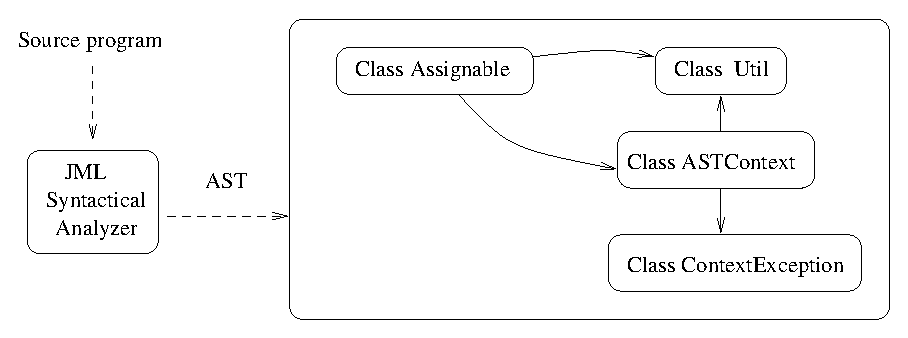
\epsfig{file=figures/schema.eps, width=9cm, clip=}
\end{center}
\caption{Structure of \modtool}
\label{fig-str-mod-tool}
\end{figure}

The tool takes as input
\java~specified files and, by using the syntactical analyzer of \jml,
figures out their Abstract Syntax Trees (ASTs) which constitute the
input of the class \texttt{Assignable}. Each rule defined in
Section~\ref{sec-syn-met-che-ass-cla} has a
corresponding representation in the class \texttt{Assignable}. Thus,
for example, the rule \textsf{(Assig)} is implemented as:

\begin{alltt}
public static boolean _mod(AST e, ASTContext currentContext)
    throws assignable.exception.ContextException\verb!{!
  if(e.getType() == JavaTokenTypes.ASSIGN)
     return in_PRIME(e.getFirstChild(),currentContext) &&
        _modFE(e.getFirstChild(),currentContext)
        _mod(e.getFirstChild().getNextSibling(),currentContext);
\verb!}!
\end{alltt}

So, whenever \modtool\ finds a \texttt{JavaTokenTypes.ASSIGN}
expression, it checks that the left expression appears in the list of
assignable locations the method is permitted to modify (method
\texttt{in\_PRIME}) and recursively calls the methods \textsf{modFE}
and \textsf{mod}, with the left and right trees of $e$, in order to do
additional checks.

As it can be seen, this method is parameterized by the expression
\texttt{e} that should be
analyzed and by the context where this expression occurs. Basically,
the context of certain instruction is constituted by the set of
locations it may modify. This context is calculated as the
addition of the parameters and the assignable locations of the method.

The class \texttt{Util}, among other functionalities, calculates
contexts, in a such way that whenever it cannot establish the
context of certain instruction, an exception
of type \texttt{ContextException} will be thrown. Furthermore, the
class \texttt{Utils} contains methods to format the
Abstract Syntax Trees returned by the \jml\ syntactical analyzer, in
order to be used by the class \texttt{Assignable}.




\subsection{Experiences using \modtool}
\label{sub-sec-usi-the-too}
In an earlier case study \cite{CatanoH02b}, we provided
specifications for a \textsc{JavaCard} purse application. These
specifications made allusion to the functional behavior of
methods (pre- and postconditions), class invariants and frame
conditions of methods. We used \escj~to check the
specifications but we could not check the assignable clauses
since \escj~do not check this at all. 

Therefore, we used \modtool~to check these clauses, thus finding some
places where these clauses do not respect the implementation. We
checked the 3 packages of the purse application, namely,
\texttt{utils}, \texttt{pacapinterfaces} and \texttt{purse}, having 27
classes, and we found 43 problems in the specification of assignable
clauses. (See~\cite{CatanoH02URL} for a full compendium).

Basically, these problems involved missing assignable clauses. The
tool
efficiently detected those problems and issued a warning
message, displaying the \textsc{AST} tree of the structure that violates
the assignable clause. 
the specification. Another important aspect of checking this purse
application constitutes the fact of having available a list of its
side-effects free methods for this application.

We present, an example of \modtool~detecting a missing assignable
clause. 
%%%%%%%
\begin{alltt}
/*@ 
  modifies intPart, decPart;
*/ 
public Decimal setValue(short i, short d) throws DecimalException\verb!{!
  if(i < 0 || d < 0 || d >= PRECISION || 
     (i == MAX_DEC_NUMBER && d != 0))
    decimal_exception.throwIt(decimal_exception.DEC_OVERFLOW);
  intPart = i;
  decPart = d;
  return this;
\verb!}!
\end{alltt}
%%%%%%%
The method \texttt{setValue} is responsible of setting the fields of
the class \texttt{Decimal}, which is a representation of an integer
part, \texttt{intPart}, and a decimal part,
\texttt{decPart}. Initially, our
assignable specification just included the 
variables \texttt{intPart} and \texttt{decPart}, since they are
directly assigned in the body of the method, but we forgot that
actually the invocation of the method \texttt{throwIt} modifies
other locations.

When using \modtool~on this method, it issues the message$:$
%%%%%%%
\begin{alltt}
[[METH,setValue]]
Warning: expression
:
:`--(
:   |--. 
:   |  |--decimal_exception
:   |  `--throwIt
:   `--.
:      |--decimal_exception
:      `--DEC_OVERFLOW
:
may contain a problem
\end{alltt}
%%%%%%%

This indicates that the invocation of the method \texttt{throwIt} in
\texttt{setValue}
may be the source of certain problem. An inspection of the
specification of the method \texttt{throwIt} shows that it
modifies the locations \texttt{decimal\_exception.instance} and
\texttt{decimal\_exception.instance.type}, and that therefore these
locations must be mentioned in the assignable clause of
\texttt{setValue}.






\section{Conclusion and future work}
\label{sec-con-and-fut-wor}
This paper presents a method to do an efficient check on assignable
clauses. In particular, this method can be used to do a quick check on 
side-effect freeness.
This method works on a syntactic basis: 
for each \java\ construct a rule is defined which checks that every
assignment or method call only modifies variables that are declared as 
\emph{assignable}. %Currently, the tool does not work with model 
%variables (specification only variables), but these could be handled
%in a similar way.

There are some limitations to our approach, in particular it does not
work in a context with aliasing. In such a case, full formal
verification is necessary, but applying our method first one finds the
simpler mistakes quickly, thus allowing to concentrate on the
essentials when verifying.
%, our
%method can miss the variable modified. Several solutions have been
%proposed for solving this problem. In~\cite{Leino98} a solution with
%\emph{Data groups} is proposed, which enables modular checking.

%Our rules, and the implementation we are done, allow one to check for
%side-efects efficiently, as no too much is spend in it. 

\subsubsection{Future work}
Our method does not keep track of newly allocated memory. Therefore,
it will reject for example this method specification for \texttt{m}
(assuming that we have a class \texttt{O} with integer field {i}):
\begin{verbatim}
//@ modifies \nothing;
m() {
 O o = new O();
 o.i = 3;
}
\end{verbatim}
To overcome this limitation, future work is to extend our method to extend the
assignable clause with the (primitively typed) fields of newly
allocated method.

\jml\ provides so-called model variables, which allows to define
specification-only variables and relate them to concrete variables by
using \texttt{represents} or \texttt{depends} clauses,
following~\cite{Leino98}. These model variables also can be mentioned
in assignable clauses. It is future work to extend the tool to
appropriately handle this.

%On the other hand, in the process of specifying abstract classes, some
%times is useful to define fields
%which \emph{represents} or \emph{depends} of certain properties of those
%classes. Due to the nature of the abstract classes it becomes not
%convenient to define these fields in an implementation
%level. \jml\ provides the construct \texttt{model} to overcome this
%difficulty. This construct allow one to define fields in a
%specification level, hence they do not have to be implemented. Besides 
%this construct, \jml\ provide the constructs
%\texttt{depends} and \texttt{represents}. Our specification does not do any 
%analyses of this type as ``it is reasonable to wait until we clarify
%the precise semantics of dependencies''\footnote{Text taken from an
%email from Gary Leavens.}.

Finally, we plan to extend the tool to give better results in the
context of aliasing and the other limitations, for example by
returning a warning if a possibly aliased variable has changed.

\bibliographystyle{plain}
\bibliography{../specification}

\end{document}
